\chapter{Gramática Emergente en Dinámica Cortical}

\label{ch:phonetics}




\iftoggle{DEBUG}{
\section{Introducción}

Dada la complejidad del lenguaje humano, se hace difícil entender cómo los infantes pueden descubrir su estructura interna para lograr comportamiento comunicativo significativo.
Independientemente de ello, los infantes alcanzan tal comportamiento exitosamente en los primeros años de vida \cite{Saffran12874}.
Algunas líneas de investigación destacan la importancia de la estructura estadística que subyace el lenguaje en general \cite{Romberg2010StatisticalLA, 10.1371/journal.pone.0177794}, mientras que otras muestran que infantes de 11 a 20 meses de edad pueden adquirir diferentes aspectos de las reglas gramaticales abstractas \cite{doi:10.1111/infa.12094, doi:10.1111/j.1467-8624.2012.01869.x}.

Muchos modelos psico-lingüísticos proponen que en el procesamiento oracional en línea, se integran diferentes tipos de restricciones muy rápido de manera coherente determinando cómo las palabras son sintacticamente combinadas en oraciones gramaticales \cite{Gibson1998-GIBCOS}.
Se propone que restricciones cualitativamente distintas como las las estructuras semánticas/conceptuales, fonológicas y sintácticas operan de manera conjunta en una unión referencial dentro del modelo discursivo \cite{Rego1993TheCB, 10.1371/journal.pone.0177794}.


%In this research, we are inspired by a psycho-linguistic model, the Unification Framework, in which unification operations during sentence comprehension take place in a parallel fashion at the semantic, syntactic and phonological levels of processing \cite{Hagoort2005OnBB}. During on-line comprehension, lexical items are processed sequentially as the time course of the input elapses. The structural frames associated with each word are combined by means of an incremental unification mechanism, in the order that the input imposes.

%In the present work, we introduce a bio-inspired neurocomputational model in which each word from the mental lexicon is associated with a structural frame. Each structural frame consists of the combination of the semantic/conceptual and phonological environment of the particular lexical item. In this model, constituent structures are established by an unification operation which consists of linking up semantic, phonological and sequential constraints correlating them repeatedly until grammar spontaneously emerges. Grammar emergence is obtained without any kind of optimization guidance beyond the correlation of the different constraints.

%The \gls{uf} \cite{Hagoort2005OnBB} proposes that only one phrasal configuration remains active among the alternative binding candidates. Such selection mechanism would be achieved by means of a lateral inhibition process between two or more alternative unification links.

%\begin{quote}
   %The outcome of the unification process is thus achieved via a selection mechanism (i.e. lateral inhibition) that ‘chooses’ between different unification options.
%\end{quote}

%In the same way, in our neurocomputational model, information coming from lateral and apical dendrites constrains the massive activation of units excited by afferent dendrites \cite{10.1371/journal.pone.0217966}. Afferent dendrites receive semantic constraints while apical dendrites receive phonological constraints. Phonologically-based implicit-learning mechanisms have been shown to serve as a precursor to later grammar learning in 4-month-old infants \cite{10.1371/journal.pone.0017920}. Lateral dendrites, on the other hand, receive information from the previous activations in the same cortical patch making the network aware of the sequence of lexical constituents along each sentence (Fig. \ref{fig:EncoderConnections}).

%\begin{figure}[h!]
    %\centering
    %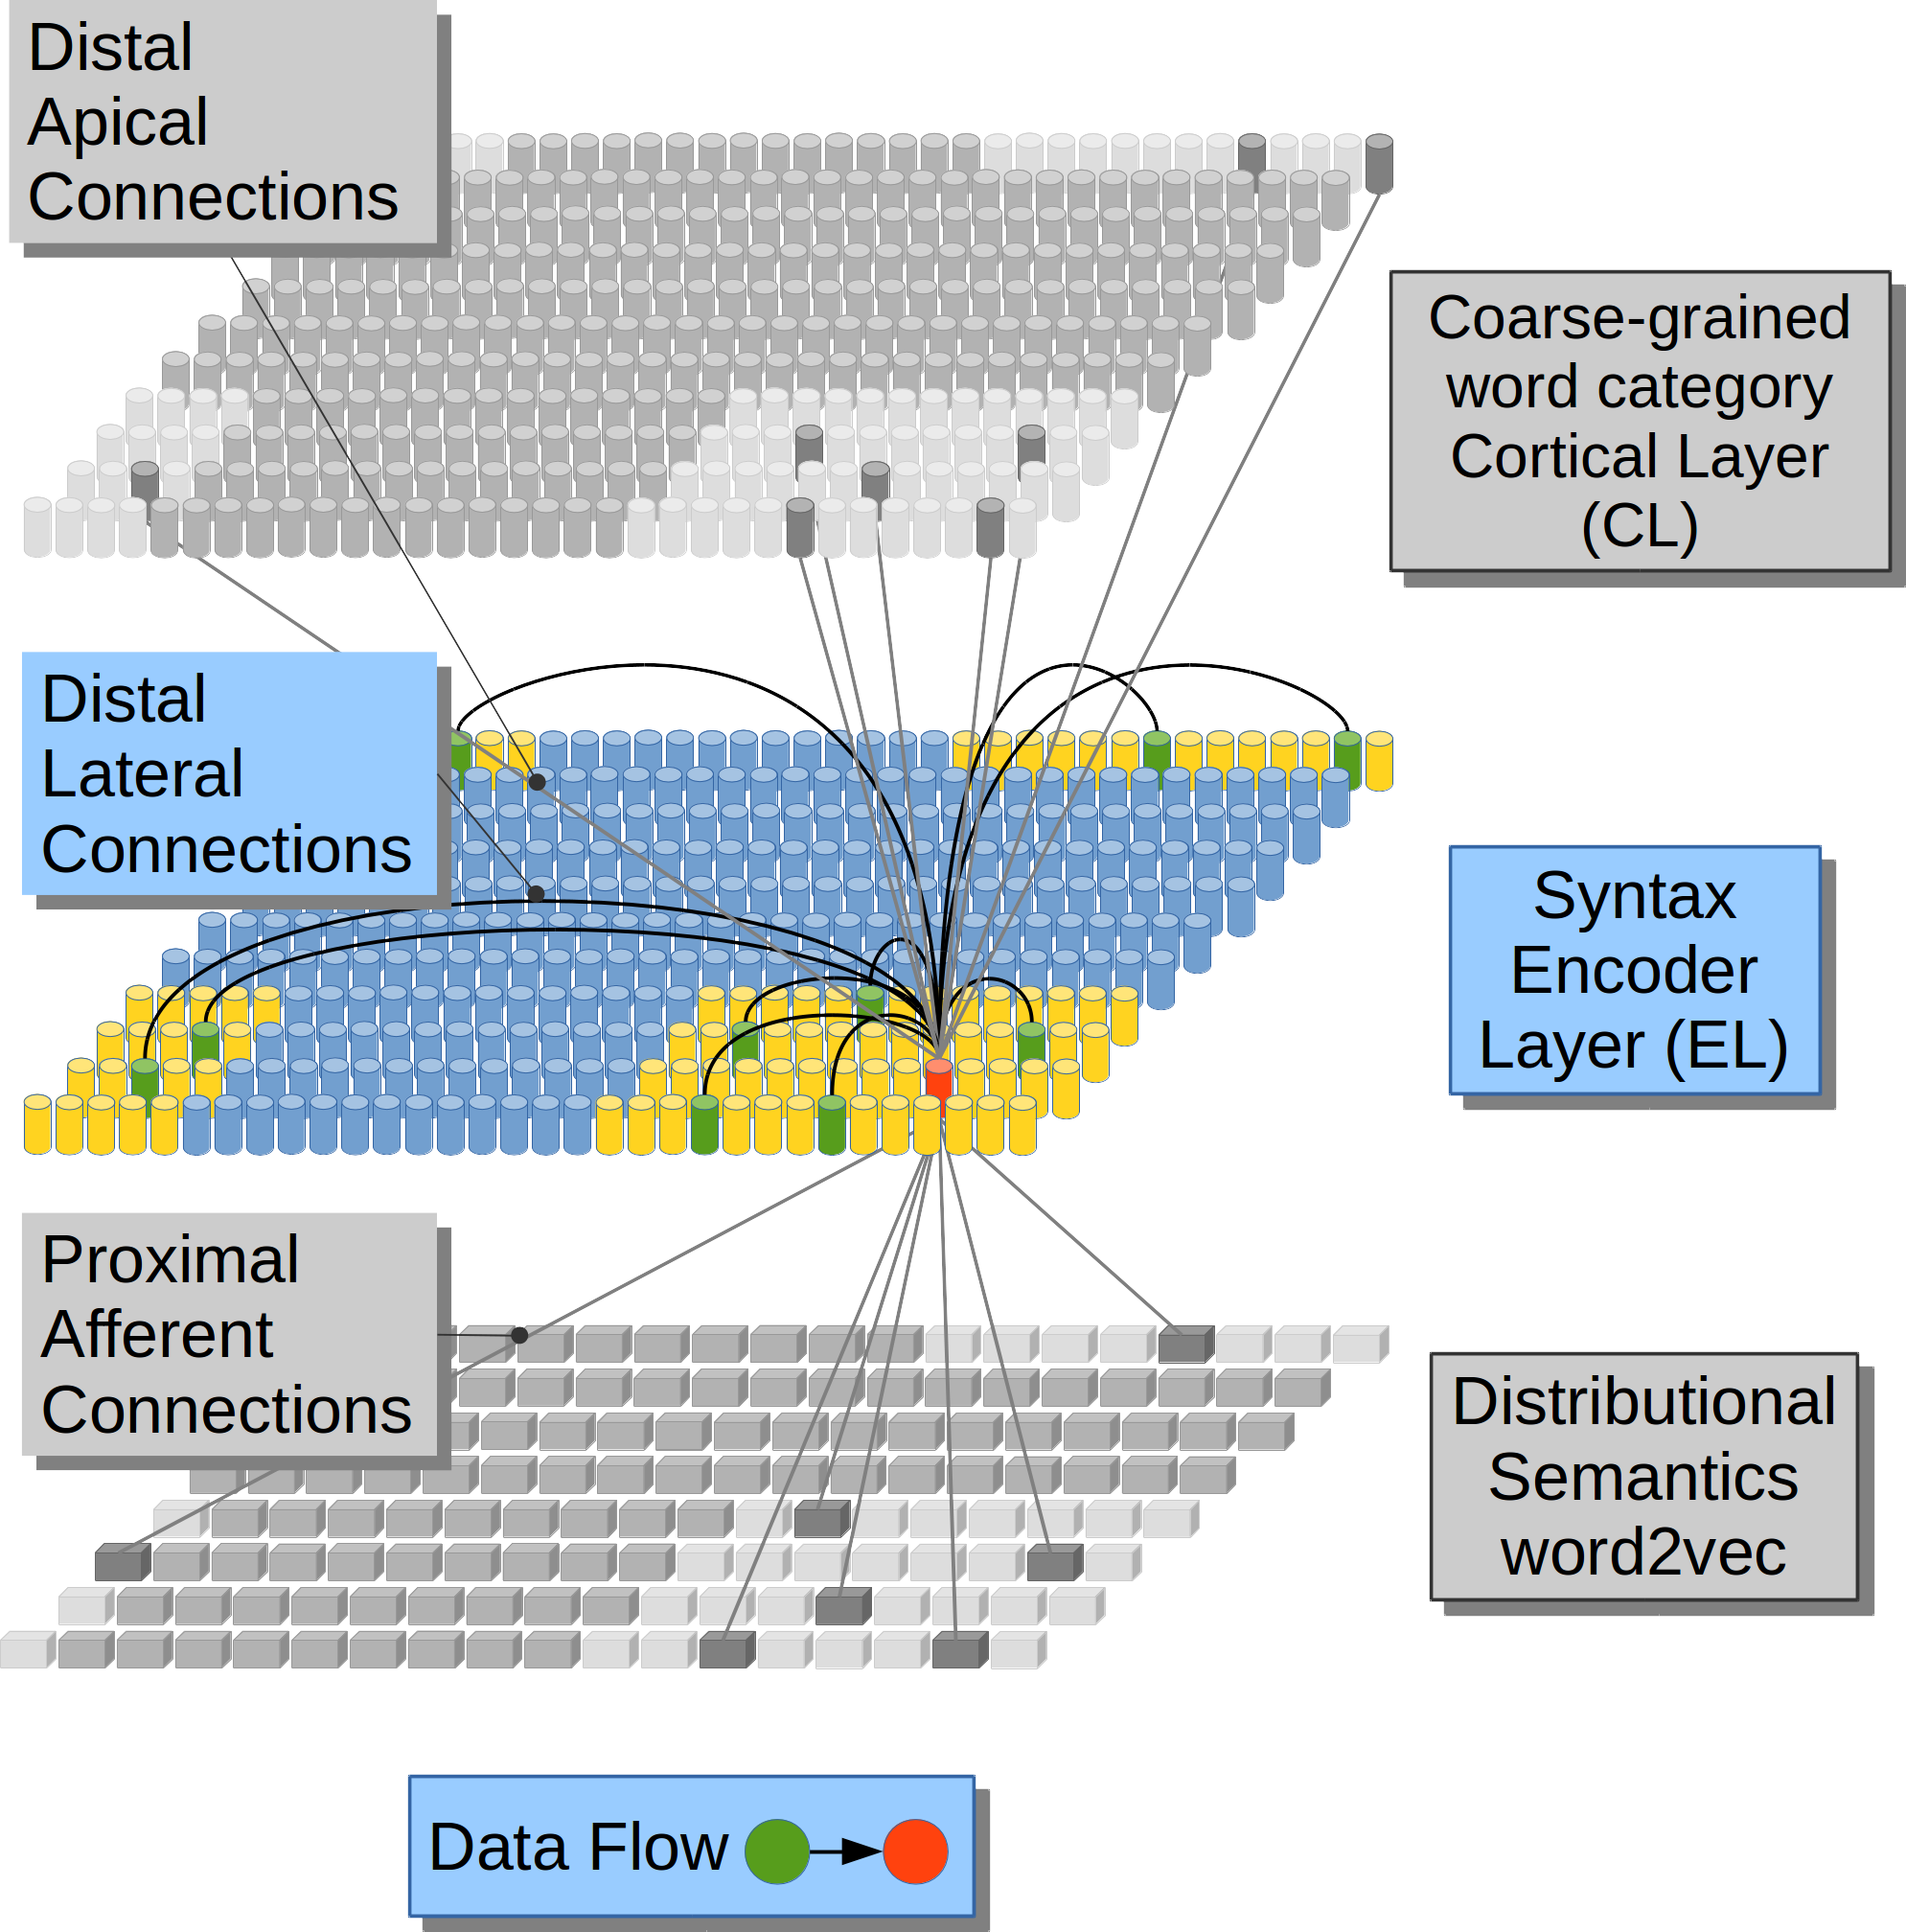
\includegraphics[width=1.0\textwidth]{EncoderConnections.png}
    %\caption{Computational implementation of the \glsfirst{uf} and its \gls{lifg} biological counterpart.
    %On the left we have the connection scheme for a \gls{cc} in the \gls{el}.
	    %Each cylinder in the \gls{el} and in the \gls{cl} represents a \gls{cc} in neural tissue.
	    %Each prism in Semantics (word2vec) represents a real valued variable.
	    %This is a visualization of a \gls{cc} (in red) and its three receptive fields (lateral in yellow and afferent and apical in light gray).
    %On the right we have the biological counterpart which is simulated by the computational implementation.
        %\glspl{ba} 47 and 45 are simulated by means of word2vec which produces semantic vectors.
        %\glspl{ba} 44 and 6 are simulated by means of \gls{sdr} activations from a fictitious \gls{cl}.
        %Finally \glspl{ba} 45 and 44 are simulated by means of the \gls{el}.
	%Brain Image adapted from \url{https://svgsilh.com/image/155655.html}}
    %\label{fig:EncoderConnections}
%\end{figure}

%We claim that semantic constraints from afferent dendrites excite clusters of neurons in a cortical patch composed by \glspl{ba} 45 and 44 which are believed to contribute to syntactic processing \cite{Pallier2522, doi:10.1152/physrev.00006.2011, doi:10.1146/annurev-neuro-071013-013847}. We simulate such cortical patch by means of a structure called \gls{el} which is depicted in Fig. \ref{fig:EncoderConnections}. The \gls{el} receives semantic constraints in its afferent dendrites from \glspl{ba} 47 and 45 which are involved in semantic processing \cite{GOUCHA2015294, DECARLI2007933, PMID:15528098, NEWMAN201051}. Semantic information tends to activate clusters of units in the \gls{el}. Such activations are massive at first, covering all the plausible lexical hypotheses that semantic information conveys. All the lexical hypotheses activated by afferent dendrites are narrowed down by distal dendrites receiving previous activations from the very same \gls{el} (lateral) and by distal dendrites receiving Phonological information (apical) from \gls{ba} 44 and part of \gls{ba} 6 which have a role in phonological processing \cite{Lee3942, PMID:27381836, HEIM2003285,
%PMID:18296070, AMUNTS200442}. Distal connections partially depolarize specific neural units in the \gls{el} which will get a running start on their activations compared to neighboring units, when afferent information arrives. Partially depolarized units will activate faster than their counterparts, inhibiting their depolarization and, in this way, preventing them from firing. By means of such strategy, the \gls{el} generates \glspl{sdr} with a 99\% of sparsity, popping up only one choice among all the alternative unification links. We propose that in such way only one phrasal configuration remains active among the alternative binding candidates.

%Thus, in the present work, we introduce a fully unsupervised approach in which constraints from different sources are correlated repeatedly until grammar naturally emerges from the statistical properties of the stimulus. Our computational model does not apply any form of optimization guidance beyond Hebbian learning. It does not backpropagate errors, nor optimize weights based on hypothetical cost functions. 

%An influential trend of compelling researches is currently trying to explain how Back-Propagation might be carried out by neural tissue in the brain \cite{WHITTINGTON2019235}. Biologically questionable aspects of the Back-Propagation algorithm such as the lack of local error representation and the need of symmetry in forward and backward weights are addressed by sound neurocomputational theories \cite{10.7554/eLife.22901, Lillicrap_2016}. Although such theories contribute with powerful arguments favoring the fact that Back-Propagation could have been implemented by evolution in cortical tissue, empirical evidence is far from conclusive. We believe there is still a long way to go before we can assure that the complex requirements imposed by \emph{credit assignament}--the ultimate goal of Back-Propagation--could be a phenomenon occuring in cortical tissue.

%In such regard, we remain cautious, keeping our model as simple as possible. We do not implement reinforcement mechanisms either. Instead, we feature strong evidence from current deep neural network approaches in which spontaneous emergence of abstract concepts seems to be a new landmark for \gls{ml}. For instance, it has been seen that biologically-inspired deep neural networks spontaneously gain number sense even when trained only to recognize objects in an image \cite{Nasreaav7903}. Moreover, using the same computational hypotheses than in the present work, our group has shown how phonetic invariance and generalization spontaneously emerges from the sequential constraints imposed by the statistical structure of the stimulus. Avoiding the utilization of optimization guidance mechanisms--such as supervision or reinforcement--we could significantly improve the \gls{svm} phonetic classification performance of stimuli seriously impaired by different levels of white noise, reverberation and changes in pitch and voices \cite{10.1371/journal.pone.0217966}.

%In the present work, we advance an improved version of the neurocomputational model previously developed in \cite{10.1371/journal.pone.0217966}. In its present form, afferent dendrites drive semantic Text Embedding information, while lateral dendrites receive sequential syntactic restrictions but, more importantly, we incorporate apical dendrites which simulate backward connectivity carrying phonological information from distant cortical patches. Backward connectivity has been seen to be prevalent in brain cortex, usually related to modulatory functions, driving effects produced by forward connections, and transcending more than one cortical level \cite{news_hidden_2018, marques_functional_2018, Chen2009ForwardAB}. Therefore, we show how our model--specifically the \gls{el}--in its current form, displays the acquisition of complex cognitive phenomena such as grammatical category, improving the \gls{svm} classification of grammatical functions within a sentence, compared to current (and powerful) word embedding representations \cite{Mikolov:2013:DRW:2999792.2999959, mikolov2013linguistic, journals/corr/abs-1301-3781}.
}{
\section{Introduction}

Given the complexity of human language, it is difficult to understand how children can discover its internal structure in order to convey meaningful communicative behavior. Nevertheless, most of them achieve such behavior successfully within the first few years of life \cite{Saffran12874}. Some lines of research highlight the importance of the statistical structure underlying language in general \cite{Romberg2010StatisticalLA, 10.1371/journal.pone.0177794}, while others show that 11 to 20-month-olds are able to acquire different aspects of abstract grammatical rules \cite{doi:10.1111/infa.12094, doi:10.1111/j.1467-8624.2012.01869.x}. 

Many psycho-linguistic models propose that in on-line sentence processing, different types of constraints are integrated very quickly in a coherent manner determining how words are systemically combined in grammatical sentences \cite{Gibson1998-GIBCOS}. It is proposed that qualitatively distinct constraints such as semantic/conceptual, phonological and syntactic structures operate alongside on a referential binding into a discourse model \cite{Rego1993TheCB, 10.1371/journal.pone.0177794}.

In this research, we are inspired by a psycho-linguistic model, the Unification Framework, in which unification operations during sentence comprehension take place in a parallel fashion at the semantic, syntactic and phonological levels of processing \cite{Hagoort2005OnBB}. During on-line comprehension, lexical items are processed sequentially as the time course of the input elapses. The structural frames associated with each word are combined by means of an incremental unification mechanism, in the order that the input imposes.

In the present work, we introduce a bio-inspired neurocomputational model in which each word from the mental lexicon is associated with a structural frame. Each structural frame consists of the combination of the semantic/conceptual and phonological environment of the particular lexical item. In this model, constituent structures are established by an unification operation which consists of linking up semantic, phonological and sequential constraints correlating them repeatedly until grammar spontaneously emerges. Grammar emergence is obtained without any kind of optimization guidance beyond the correlation of the different constraints.

The \gls{uf} \cite{Hagoort2005OnBB} proposes that only one phrasal configuration remains active among the alternative binding candidates. Such selection mechanism would be achieved by means of a lateral inhibition process between two or more alternative unification links.

\begin{quote}
   The outcome of the unification process is thus achieved via a selection mechanism (i.e. lateral inhibition) that ‘chooses’ between different unification options.
\end{quote}

In the same way, in our neurocomputational model, information coming from lateral and apical dendrites constrains the massive activation of units excited by afferent dendrites \cite{10.1371/journal.pone.0217966}. Afferent dendrites receive semantic constraints while apical dendrites receive phonological constraints. Phonologically-based implicit-learning mechanisms have been shown to serve as a precursor to later grammar learning in 4-month-old infants \cite{10.1371/journal.pone.0017920}. Lateral dendrites, on the other hand, receive information from the previous activations in the same cortical patch making the network aware of the sequence of lexical constituents along each sentence (Fig. \ref{fig:EncoderConnections}).

\begin{figure}[h!]
    \centering
    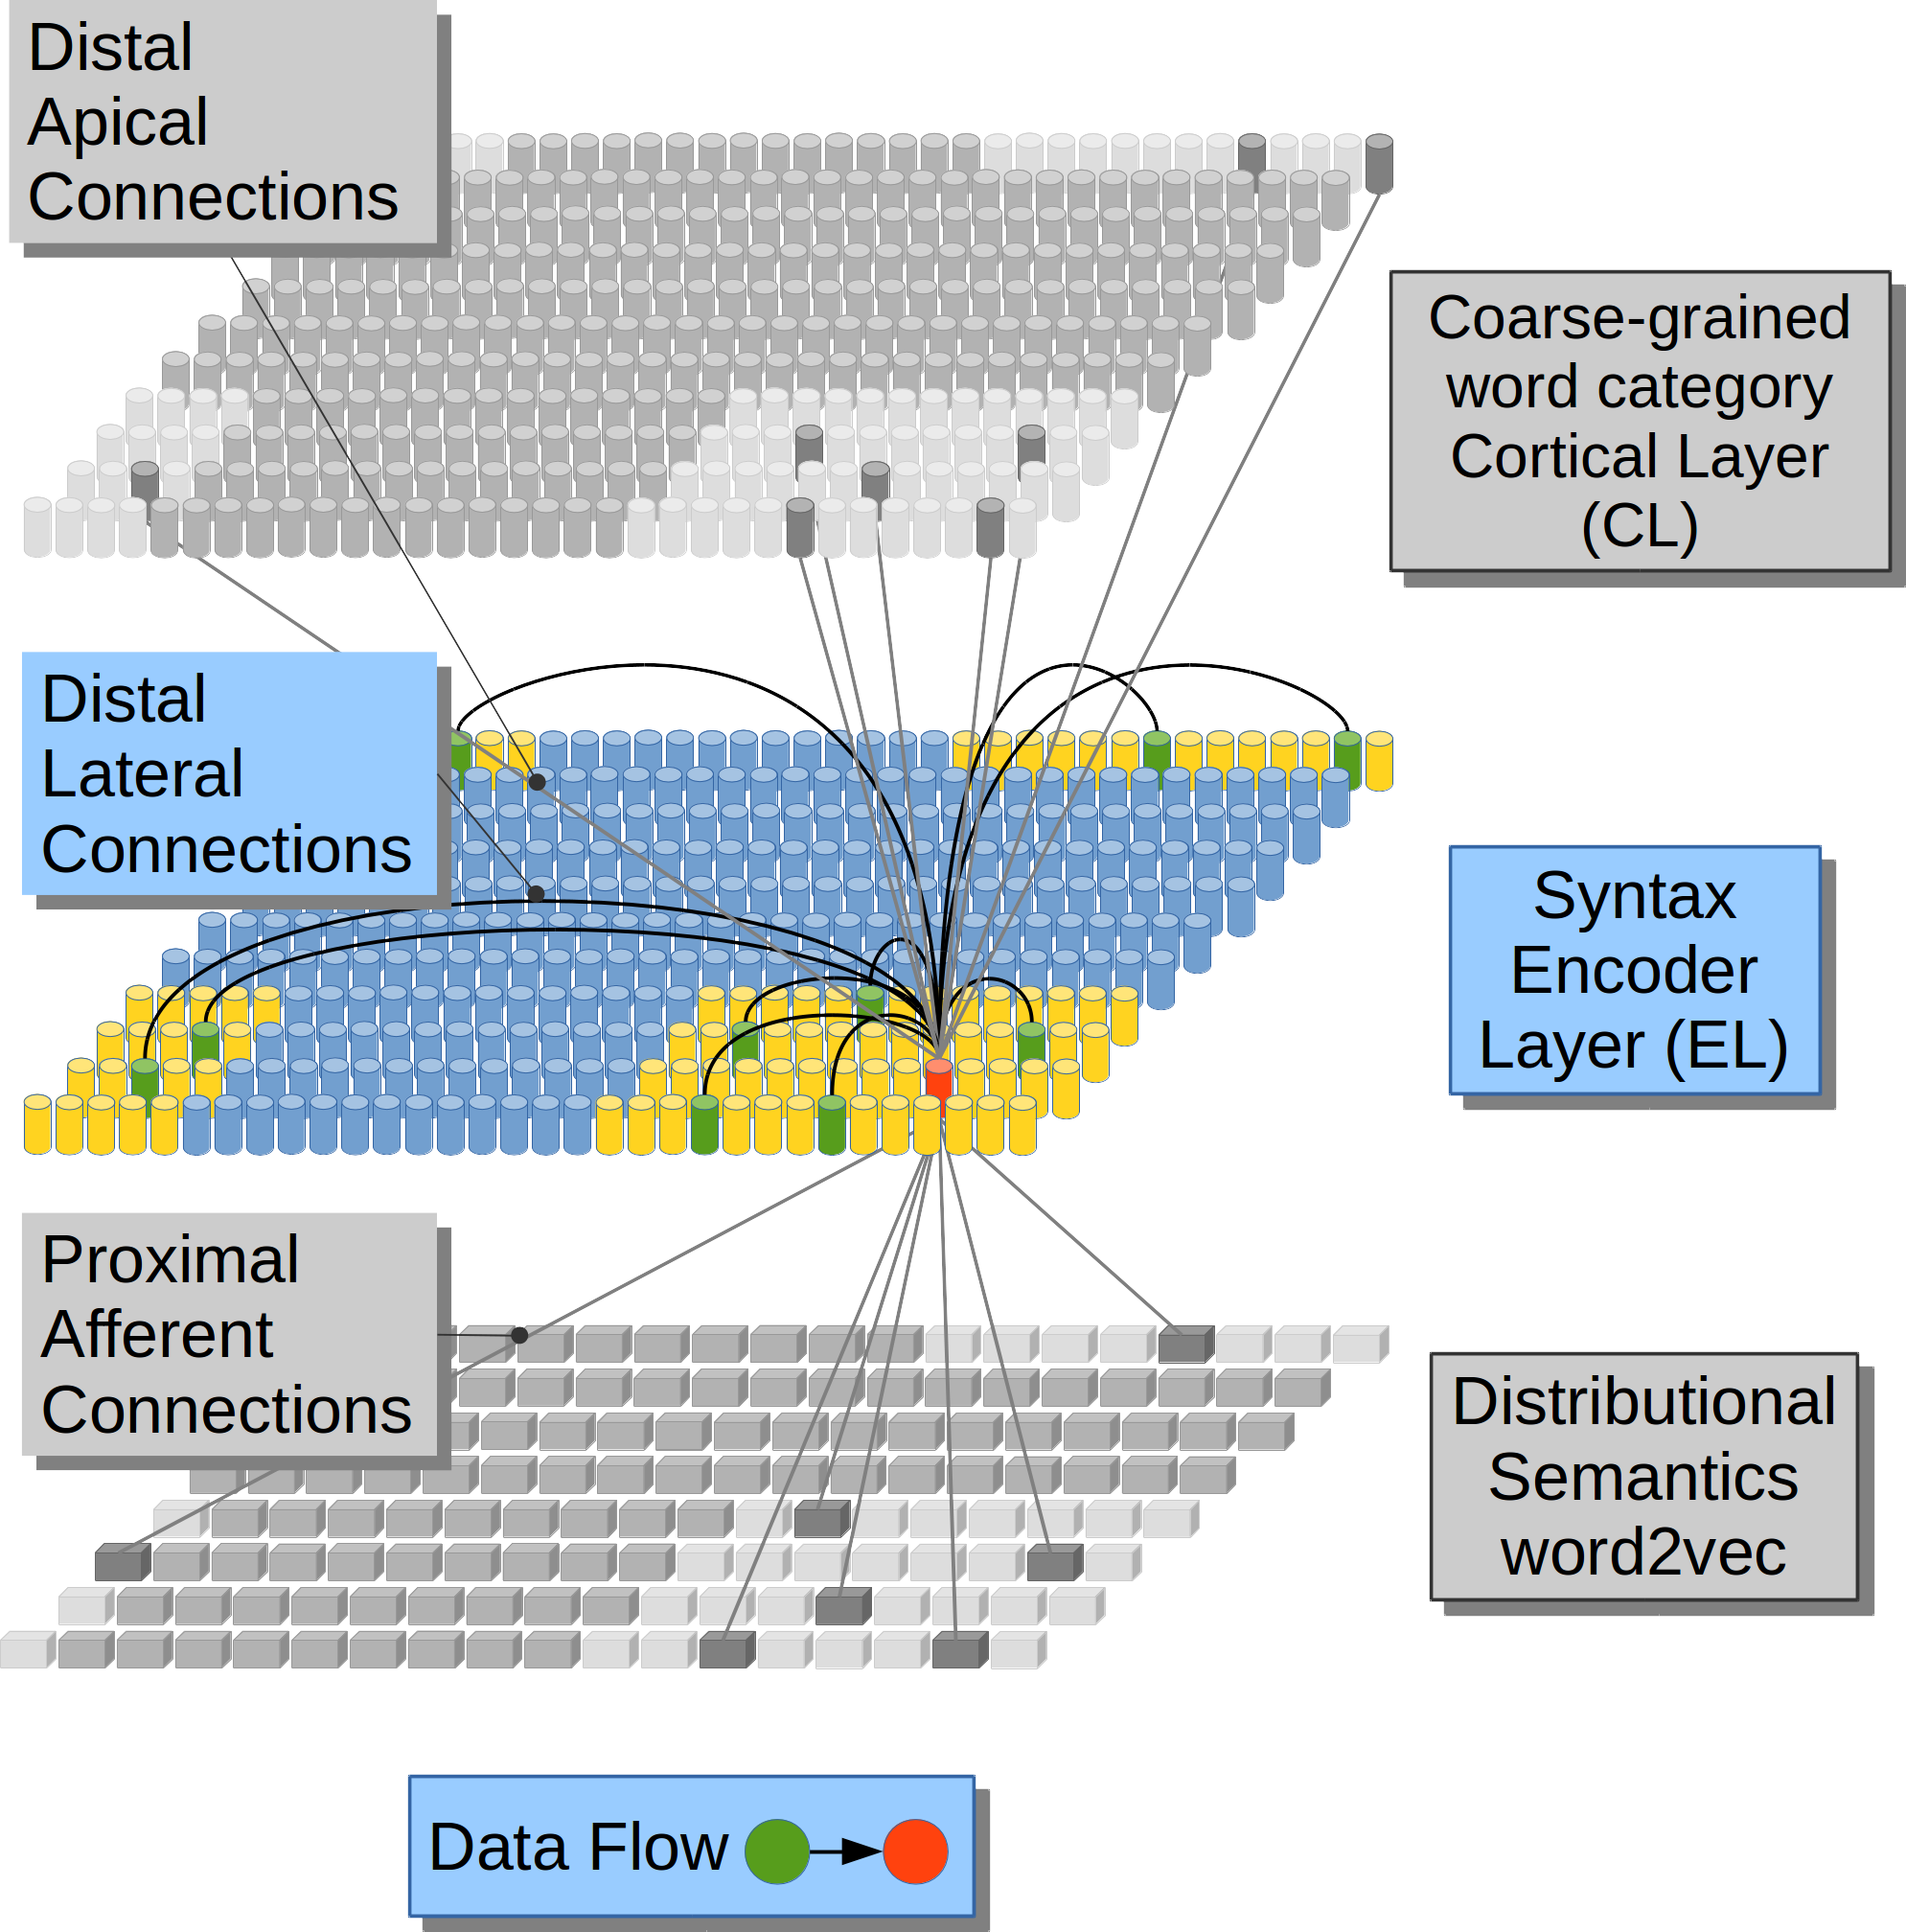
\includegraphics[width=1.0\textwidth]{EncoderConnections.png}
    \caption{Computational implementation of the \glsfirst{uf} and its \gls{lifg} biological counterpart.
    On the left we have the connection scheme for a \gls{cc} in the \gls{el}.
	    Each cylinder in the \gls{el} and in the \gls{cl} represents a \gls{cc} in neural tissue.
	    Each prism in Semantics (word2vec) represents a real valued variable.
	    This is a visualization of a \gls{cc} (in red) and its three receptive fields (lateral in yellow and afferent and apical in light gray).
    On the right we have the biological counterpart which is simulated by the computational implementation.
        \glspl{ba} 47 and 45 are simulated by means of word2vec which produces semantic vectors.
        \glspl{ba} 44 and 6 are simulated by means of \gls{sdr} activations from a fictitious \gls{cl}.
        Finally \glspl{ba} 45 and 44 are simulated by means of the \gls{el}.
	Brain Image adapted from \url{https://svgsilh.com/image/155655.html}}
    \label{fig:EncoderConnections}
\end{figure}

We claim that semantic constraints from afferent dendrites excite clusters of neurons in a cortical patch composed by \glspl{ba} 45 and 44 which are believed to contribute to syntactic processing \cite{Pallier2522, doi:10.1152/physrev.00006.2011, doi:10.1146/annurev-neuro-071013-013847}. We simulate such cortical patch by means of a structure called \gls{el} which is depicted in Fig. \ref{fig:EncoderConnections}. The \gls{el} receives semantic constraints in its afferent dendrites from \glspl{ba} 47 and 45 which are involved in semantic processing \cite{GOUCHA2015294, DECARLI2007933, PMID:15528098, NEWMAN201051}. Semantic information tends to activate clusters of units in the \gls{el}. Such activations are massive at first, covering all the plausible lexical hypotheses that semantic information conveys. All the lexical hypotheses activated by afferent dendrites are narrowed down by distal dendrites receiving previous activations from the very same \gls{el} (lateral) and by distal dendrites receiving Phonological information (apical) from \gls{ba} 44 and part of \gls{ba} 6 which have a role in phonological processing \cite{Lee3942, PMID:27381836, HEIM2003285,
PMID:18296070, AMUNTS200442}. Distal connections partially depolarize specific neural units in the \gls{el} which will get a running start on their activations compared to neighboring units, when afferent information arrives. Partially depolarized units will activate faster than their counterparts, inhibiting their depolarization and, in this way, preventing them from firing. By means of such strategy, the \gls{el} generates \glspl{sdr} with a 99\% of sparsity, popping up only one choice among all the alternative unification links. We propose that in such way only one phrasal configuration remains active among the alternative binding candidates.

Thus, in the present work, we introduce a fully unsupervised approach in which constraints from different sources are correlated repeatedly until grammar naturally emerges from the statistical properties of the stimulus. Our computational model does not apply any form of optimization guidance beyond Hebbian learning. It does not backpropagate errors, nor optimize weights based on hypothetical cost functions. 

An influential trend of compelling researches is currently trying to explain how Back-Propagation might be carried out by neural tissue in the brain \cite{WHITTINGTON2019235}. Biologically questionable aspects of the Back-Propagation algorithm such as the lack of local error representation and the need of symmetry in forward and backward weights are addressed by sound neurocomputational theories \cite{10.7554/eLife.22901, Lillicrap_2016}. Although such theories contribute with powerful arguments favoring the fact that Back-Propagation could have been implemented by evolution in cortical tissue, empirical evidence is far from conclusive. We believe there is still a long way to go before we can assure that the complex requirements imposed by \emph{credit assignament}--the ultimate goal of Back-Propagation--could be a phenomenon occuring in cortical tissue.

In such regard, we remain cautious, keeping our model as simple as possible. We do not implement reinforcement mechanisms either. Instead, we feature strong evidence from current deep neural network approaches in which spontaneous emergence of abstract concepts seems to be a new landmark for \gls{ml}. For instance, it has been seen that biologically-inspired deep neural networks spontaneously gain number sense even when trained only to recognize objects in an image \cite{Nasreaav7903}. Moreover, using the same computational hypotheses than in the present work, our group has shown how phonetic invariance and generalization spontaneously emerges from the sequential constraints imposed by the statistical structure of the stimulus. Avoiding the utilization of optimization guidance mechanisms--such as supervision or reinforcement--we could significantly improve the \gls{svm} phonetic classification performance of stimuli seriously impaired by different levels of white noise, reverberation and changes in pitch and voices \cite{10.1371/journal.pone.0217966}.

In the present work, we advance an improved version of the neurocomputational model previously developed in \cite{10.1371/journal.pone.0217966}. In its present form, afferent dendrites drive semantic Text Embedding information, while lateral dendrites receive sequential syntactic restrictions but, more importantly, we incorporate apical dendrites which simulate backward connectivity carrying phonological information from distant cortical patches. Backward connectivity has been seen to be prevalent in brain cortex, usually related to modulatory functions, driving effects produced by forward connections, and transcending more than one cortical level \cite{news_hidden_2018, marques_functional_2018, Chen2009ForwardAB}. Therefore, we show how our model--specifically the \gls{el}--in its current form, displays the acquisition of complex cognitive phenomena such as grammatical category, improving the \gls{svm} classification of grammatical functions within a sentence, compared to current (and powerful) word embedding representations \cite{Mikolov:2013:DRW:2999792.2999959, mikolov2013linguistic, journals/corr/abs-1301-3781}.
}
















\iftoggle{DEBUG}{
\section{Materiales y métodos}
}{
\section{Materials and methods}
}

















\iftoggle{DEBUG}{
\subsection{Modelo Computacional}

}{
\subsection{Computational Model}

We propose a computational approach inspired in the biology of the mammalian neocortex which simulates a patch of cortical tissue and incorporates columnar organization, spontaneous micro-columnar formation, \glspl{sdr} derived from partial \gls{nmda} depolarization, and adaptation to contextual activations. We simulate pyramidal cells with proximal connections from afferent dendritic branches and distal connections from lateral and apical dendritic branches \cite{10.1371/journal.pone.0217966}.

Information from distal dendritic branches--which is lateral and apical--produces, in advance, a partial \gls{nmda} depolarization in some cell units in a \gls{cc}  (Fig. \ref{fig:EncoderConnections}). On the other hand, information from proximal dendritic branches--which is afferent-- produces a complete depolarization of a cluster of cell units in a \gls{cc}, but in the event that enough afferently excited units have already been partially depolarized by lateral and/or apical dendrites, such units would fire before inhibiting other units in the cluster and preventing them from firing. With this mechanism, only a reduced number of units become active, producing a sparse pattern of activation in our model. This neurocomputational theory has been introduced in \cite{10.3389/fncir.2016.00023}, showing continuous online and unsupervised sequence learning capabilities \cite{Cui:2016:COS:3030654.3030660}.

Some important remarks in reference to this computational approach are: (i) proximal afferent dendrites do not determine a neuron to fire, instead, they bias its probability of doing so, (ii) distal dendritic branches are independent computing elements that contribute to somatic firing by means of dendritic spikes, and (iii) prediction failures in the network produce a phenomenon called \gls{mfe} which manifests with the activation of many neurons in a \gls{cc} impairing \glspl{sdr} formation \cite{10.1371/journal.pone.0217966}.

In reference to the random nature imprinted in the computational approach, previous studies have already incorporated stochastic forces to biologically plausible models of neuronal dynamics \cite{harrison_l.m_stochastic_2005}. In addition, the autonomy of neural dendrites as independent elements of computation has already been posed, showing that neuronal dendrites exhibit a range of linear and nonlinear mechanisms that allow them to implement elementary computations \cite{poirazi_dendritic_2015, PAYEUR201978}. Finally \glspl{mfe} in the model explain integration phenomena in which a combination of different constraints converges incoherently and produces the massive activation of a neuron cluster in the \glspl{cc} of the \gls{el}. When the \gls{el} cannot fluently integrate information coming from different linguistic constraints, it activates more hypotheses--i.e more phrasal configurations--as to be able to easily fuse subsequent information coming within the sequential sentence context. Such arguments are inspired by biological correlates, observed as \gls{erps} \cite{Hagoort2003InterplayBS}.

An activation phenomenon such as the \glsfirst{mfe} impedes \glspl{sdr} formation. However, when the \gls{el} correctly predicts the sequential stream of information coming from different constraints, it continuously produces \glspl{sdr} and the sequential activation runs smoothly. \glspl{sdr} exhibit interesting mathematical properties which give them high noise rejection and fault tolerance \cite{DBLP:journals/corr/AhmadH15}. It has been shown that the brain uses sparse patterns of activation to process information in all mammals, from mice to humans \cite{barth_experimental_2012}.
}






\iftoggle{DEBUG}{
\subsection{Restricciones Semánticas Aferentes}

}{
\subsection{Afferent Semantic Constraints}

We generate semantic constraints using Word Embedding approaches. Word Embedding is a set of \gls{nlp} techniques in which words or phrases from a vocabulary are mapped to vectors of real numbers. We specifically use word2vec which takes a large corpus of text as input and produces a vector space that usually has several hundred dimensions. Each word in the corpus is assigned to a corresponding vector in the space. The main hypothesis is that words which recurrently appear in proximal positions in the text will be located proximally in the semantic space (vector space). The output of such model is a semantic multi-dimensional space with compelling semantic properties \cite{mikolov2013linguistic, journals/corr/abs-1301-3781, Mikolov:2013:DRW:2999792.2999959}. In this paper we used pre-trained vectors obtained from part of Google News dataset (about 100 billion words). The model contains 300-dimensional vectors for 3 million words and phrases \cite{noauthor_google_nodate}.

We implemented afferent dendrites by means of \glspl{som} \cite{Kohonen:1988:SFT:65669.104428, Kohonen1989SelforganizationAA}. Each \gls{cc} in the \gls{el} simulates proximal afferent dendrites using a \gls{som} as shown in Figs. \ref{fig:EncoderProximalConnections} A and \ref{fig:EncoderProximalConnections} B. Each \gls{cc} receives a reduced sample from the word2vec components.

\begin{figure}[h!]
    \centering
    %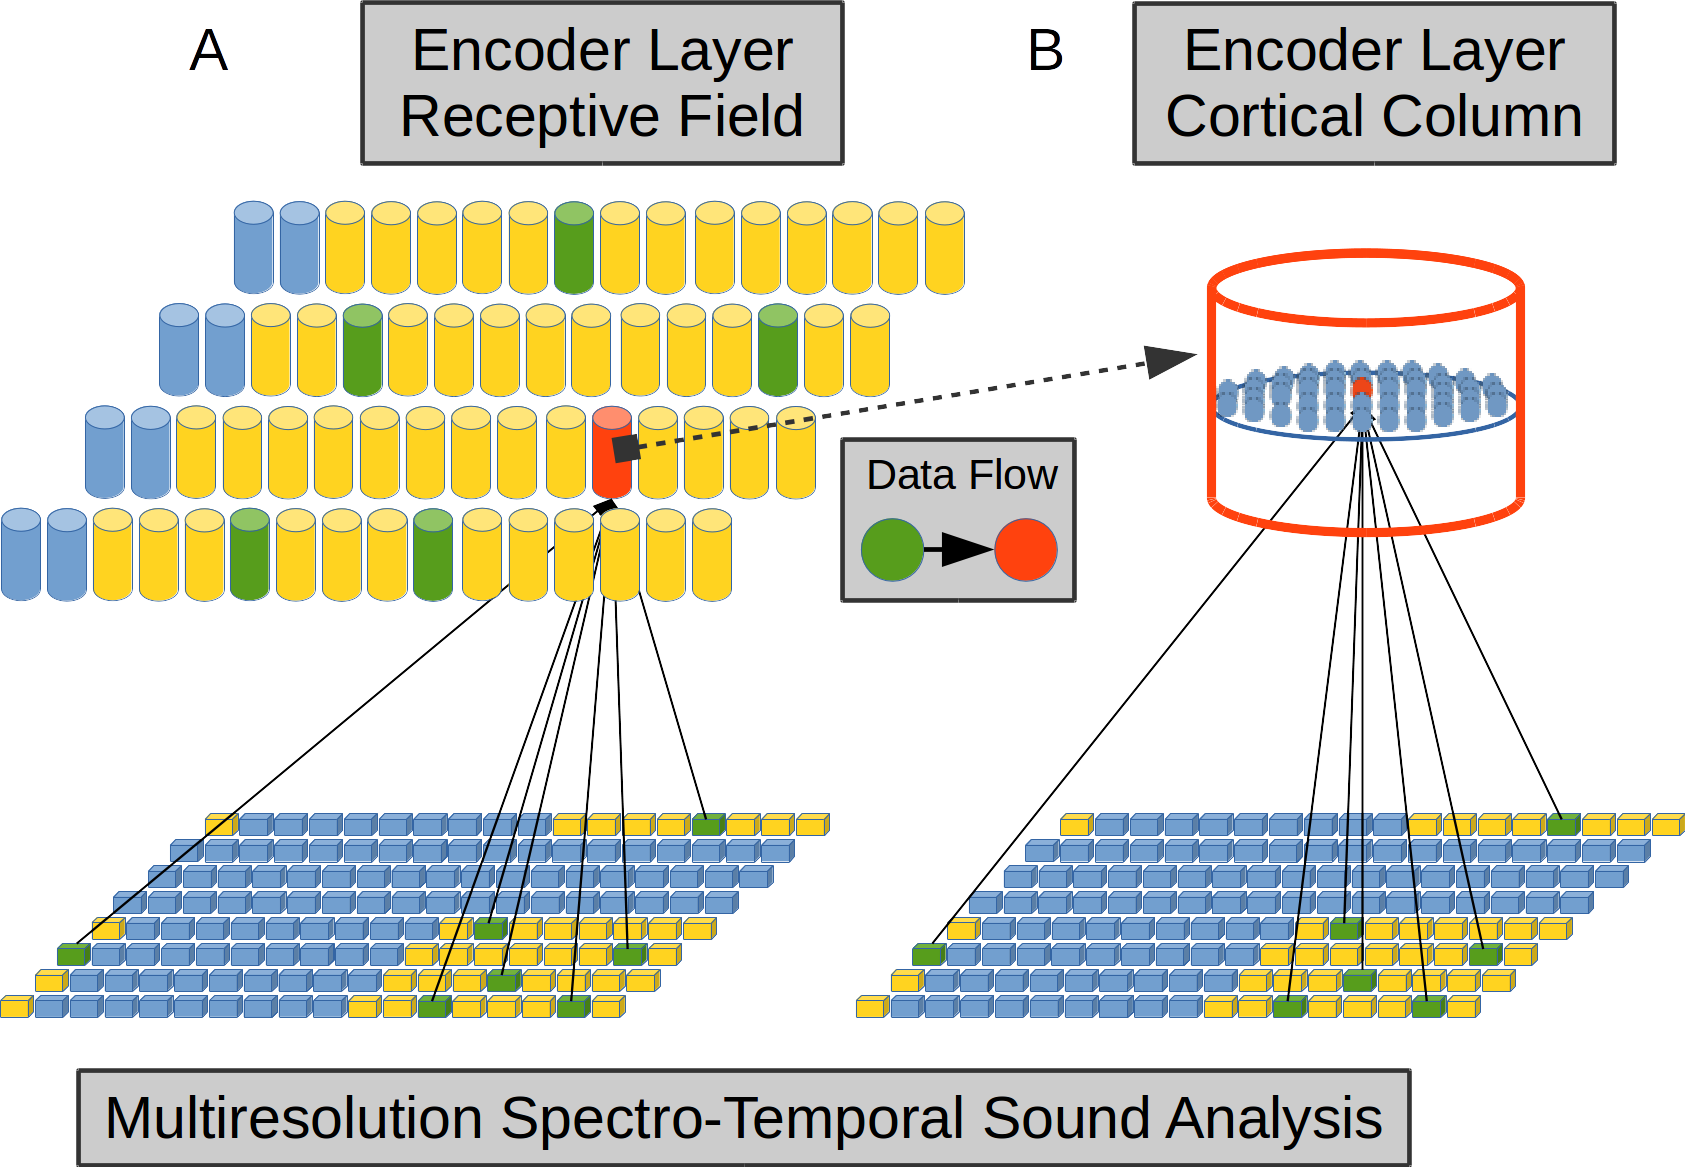
\includegraphics[width=0.8\textwidth]{EncoderProximalConnections.png}
    \caption{\glsfirst{el} proximal afferent connections. Each \gls{cc} in the \gls{el}--exemplified here in red--has its receptive field over the word2vec semantic space--in yellow.
    (A) A set of word2vec components--in green inside the receptive field--is randomly chosen to be connected with a \gls{cc}.
    (B) Each neural unit in a \gls{cc} is connected with the same set of word2vec components.}
    %(C) Each \gls{cc} set of afferent dendrites is simulated by means of a \gls{som}.
    %(D) The \gls{som} adapts to the word2vec semantic sub-space.}
    \label{fig:EncoderProximalConnections}
\end{figure}

Figs. \ref{fig:CorticalColumnSOM} and \ref{fig:CorticalColumnTrainedSOM} show the relationship between the word2vec semantic space and each \gls{cc} in the \gls{el}. In Fig. \ref{fig:CorticalColumnSOM} the \gls{cc} afferent dendrites are in their initial state and its corresponding semantic sub-space sampled from word2vec is represented by several words scattered in the background.
 
\begin{figure}[h!]
    \centering
    %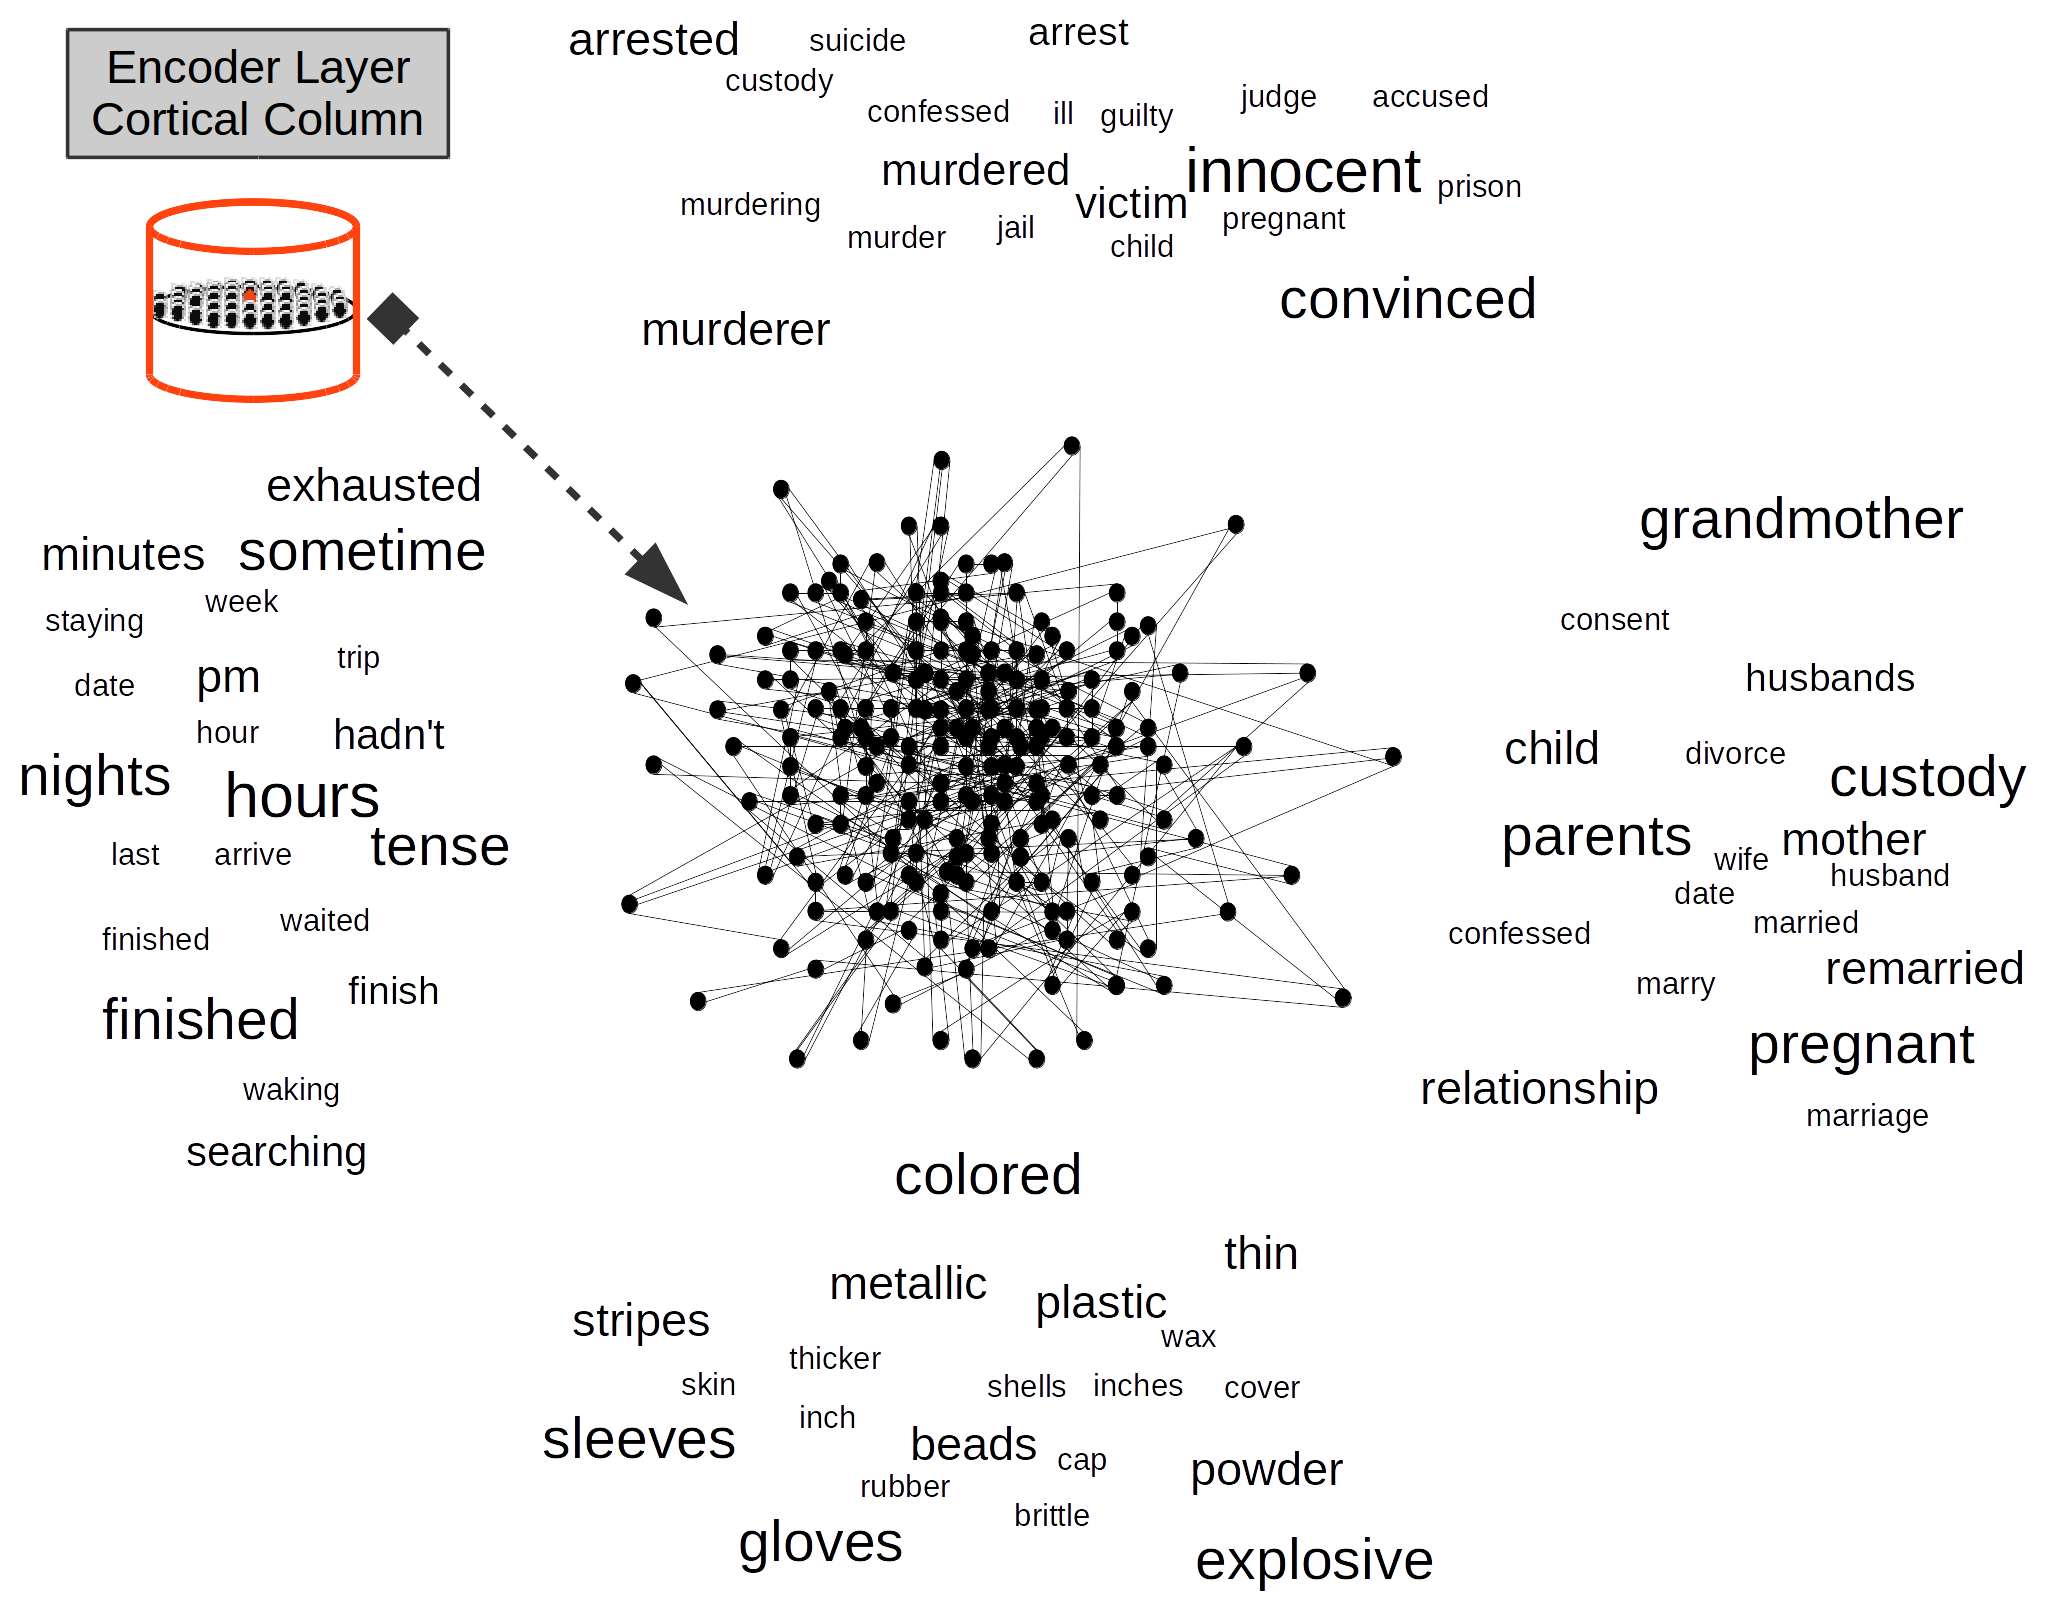
\includegraphics[width=0.9\textwidth]{CorticalColumnSOM.png}
    \caption{\glsfirst{el} \glsfirst{cc} and its proximal afferent connections represented by a \glsfirst{som}. Each \gls{cc} in the \gls{el}--exemplified here in red--has its receptive field over word2vec as a semantic sub-space represented by words scattered in the background. \gls{som} weights are in their initial state.}
    \label{fig:CorticalColumnSOM}
\end{figure}
 
 

Each set of afferent connections in a \gls{cc} determines a two-dimensional lattice of 15 by 15 neural units. The sampled semantic sub-space has 31 real valued components. In Fig. \ref{fig:CorticalColumnTrainedSOM}--once \gls{cc} afferent dendrites have been trained--the neural lattice distributes its neural units throughout the semantic sub-space. In such case, each word in the semantic sub-space will have its neural resource representation and words with semantic proximity in the semantic sub-space will be represented by neural resources with physical proximity in the lattice. The neighborhood preservation of self-organizing feature maps is an important property which turns out to be useful to preserve the original sub-space semantic relationships in the new space in the lattice of a \gls{cc} in the cortex \cite{557663}.


\begin{figure}[h!]
    \centering
    %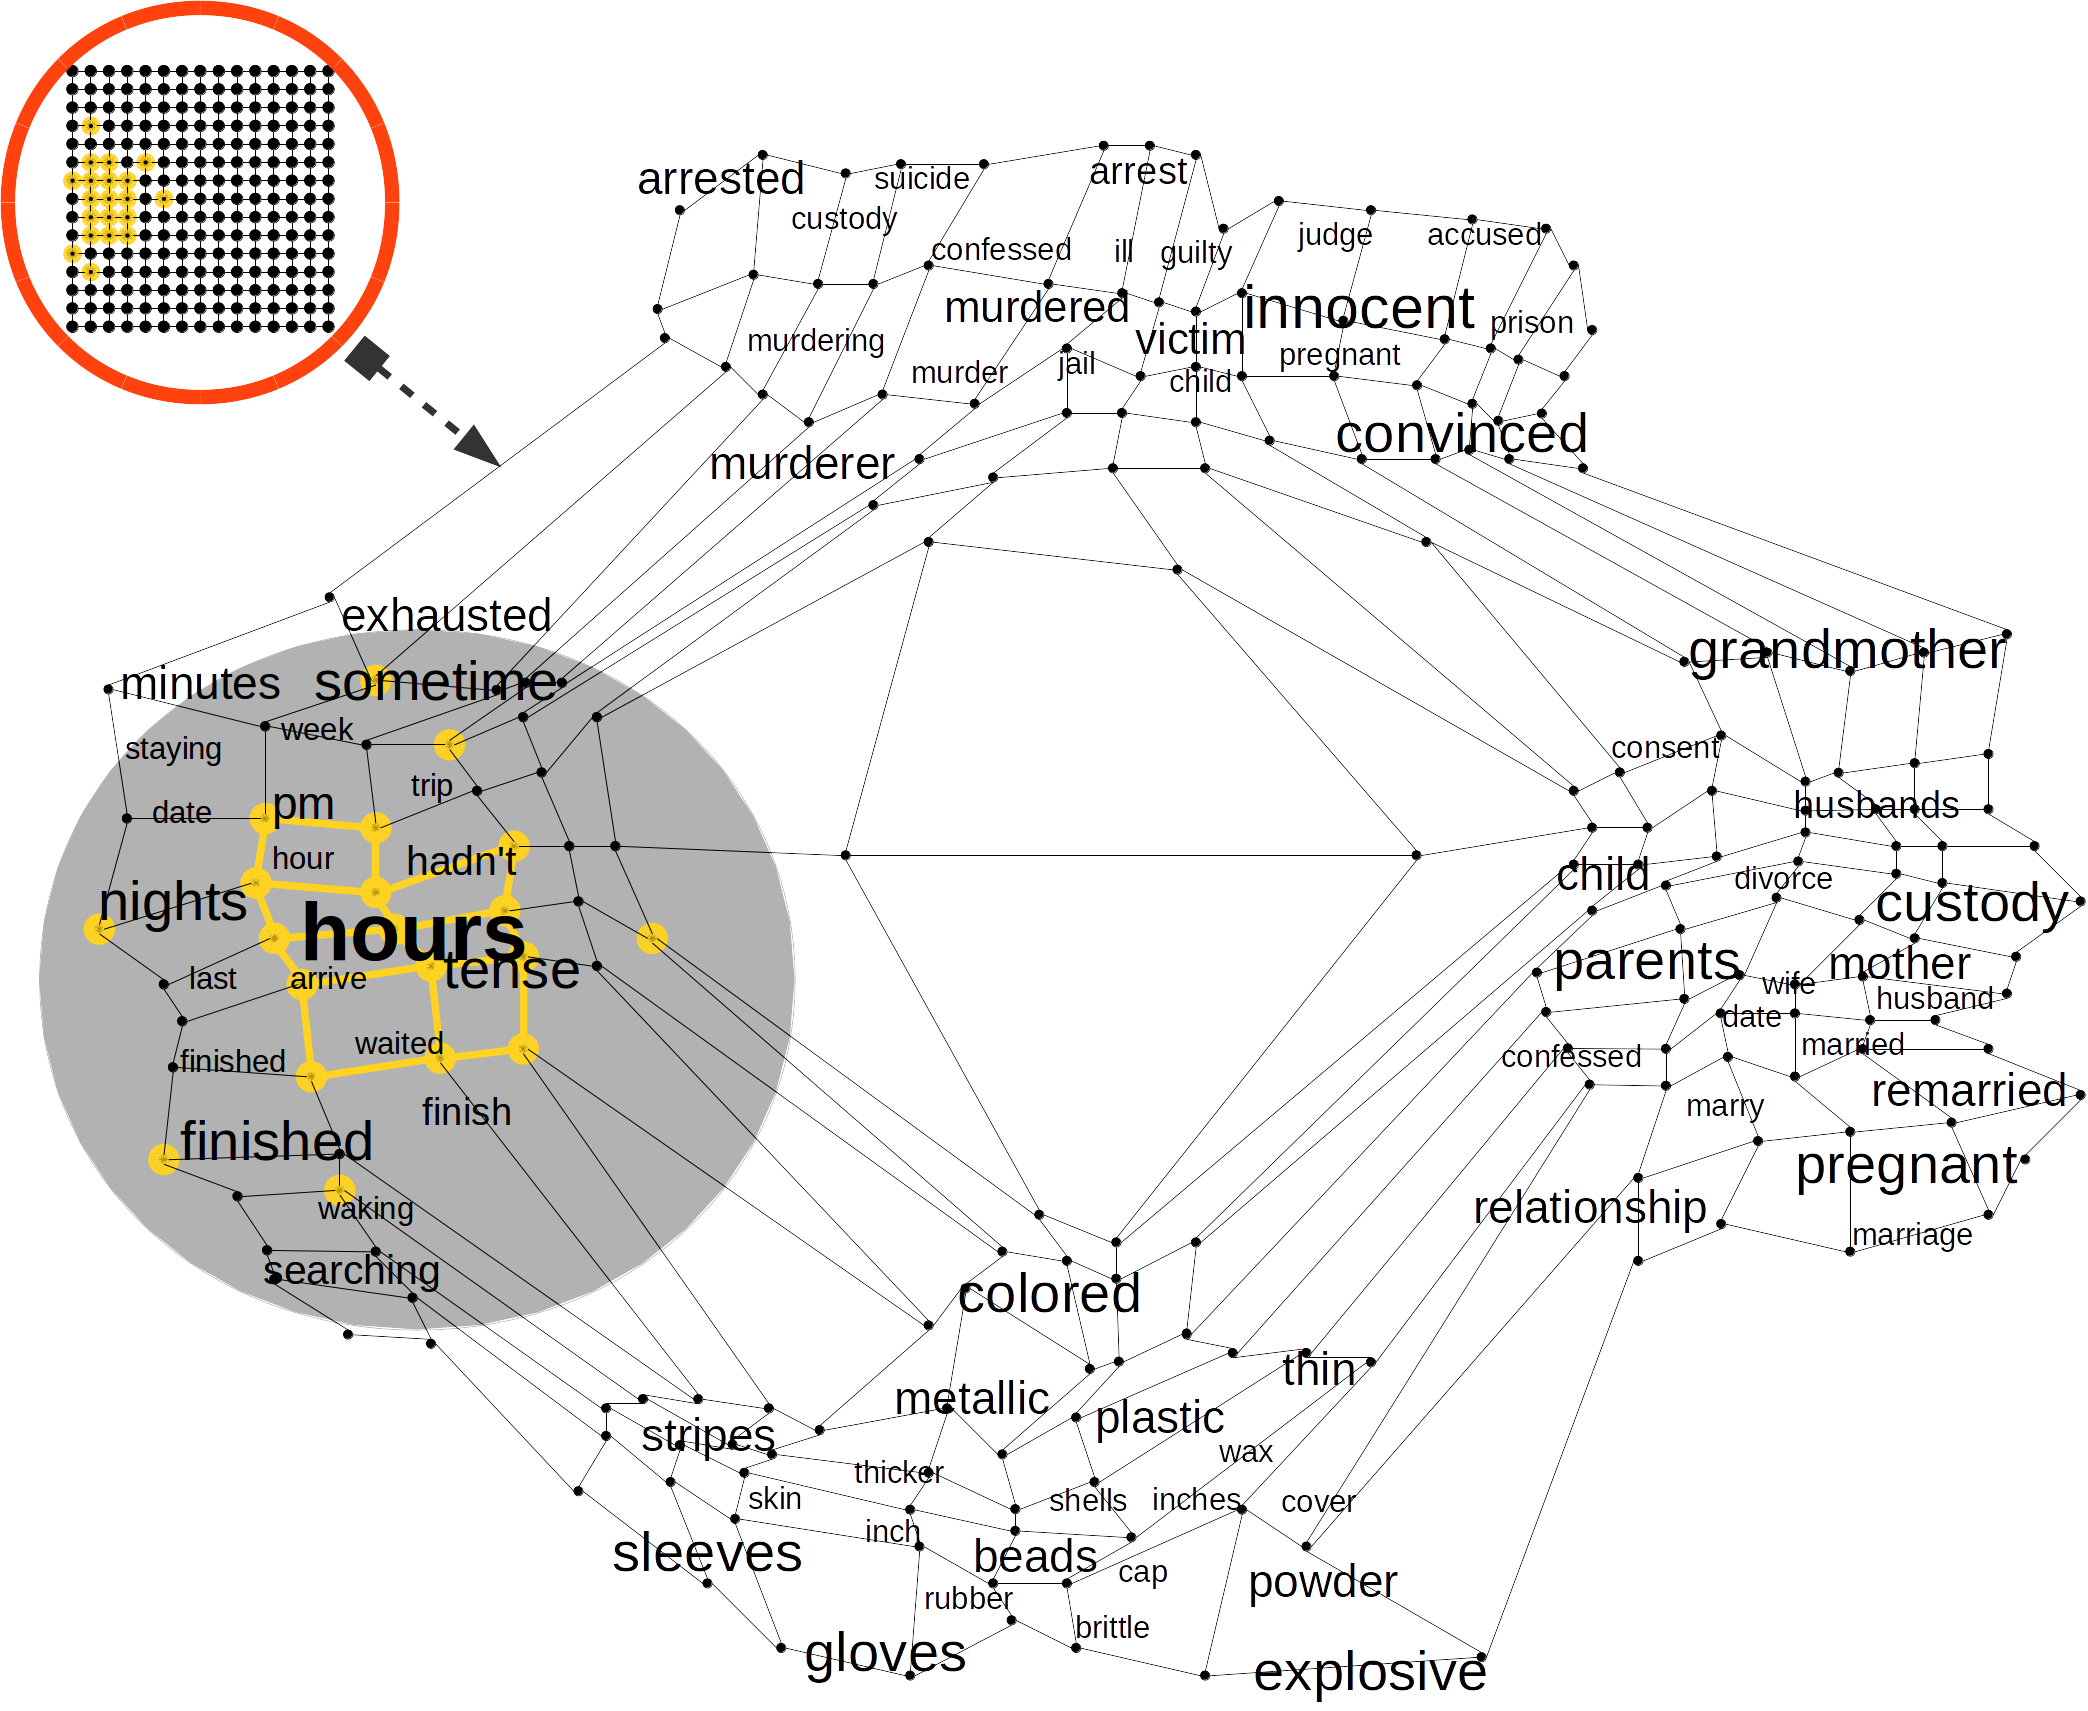
\includegraphics[width=0.9\textwidth]{CorticalColumnTrainedSOM.png}
    \caption{A trained \glsfirst{som} in a \glsfirst{cc} proximal afferent connections. The \gls{som} is a bi-dimensional lattice of 225 neural units (15 by 15 neural units). The \gls{som} adapts to represent the word2vec semantic sub-space. After trained, a \gls{som} in a \gls{cc} distributes its neural units throughout the semantic sub-space sampled from word2vec. The \gls{som} algorithm keeps the semantic topology of the original semantic sub-space imprinted in the lattice of neural units. Each word in the semantic sub-space has its neural representation and words with more semantic similarity are represented by neural units with a high physical proximity in the lattice.}
    \label{fig:CorticalColumnTrainedSOM}
\end{figure}




Once afferent dendrites have learned the statistical distribution immersed in the different semantic sub-spaces, each \gls{cc} in the \gls{el} has its private representation of its semantic sub-space from word2vec. The advent of the semantic representation from certain word in word2vec establishes a pattern of activation in a cluster of neural units inside each \gls{cc} (Fig. \ref{fig:CorticalColumnTrainedSOM}). In this way, each semantic constraint from word2vec will be represented in a distributed way throughout the \gls{el}. The semantic representation of each word will activate a cluster of neural units in each \gls{cc}, and the semantic content of such word will be distributed in the cortical patch simulated by the \gls{el}. Significant evidence shows that the semantic content of words is distributed across cortical tissue \cite{huth_natural_2016}. For example, a word like \emph{top} can not only activate a region related with clothing and appearance, but it can also activate a region related with numbers and measurements and perhaps a region related with buildings and places. On the other hand, it has also been shown that words with similar semantic content are mapped in proximal regions of the cortex \cite{pub.1005704802}. For instance, in the right temporo-parietal junction a small patch of cortex responds to words like \emph{wife, mother, pregnant, family, friends, brother} etc, while a very near patch responds to words like \emph{family} and \emph{wife} but also responds to--in certain way semantically related--words like \emph{house, roommates, household} and \emph{owner}. There are compelling brain-inspired computational approaches which use \glspl{sdr} to simulate how cortical brain activation represents the semantic content of words \cite{DBLP:journals/corr/Webber15}.

In Fig. \ref{fig:CorticalColumnTrainedSOM} we illustrate how the word \textbf{\texttt{hours}} could activate a cluster of neural units which are representative of time phenomena such as \texttt{pm, hour} and \texttt{sometime}, but it could also  activate units which represent semantically related phenomena such as \texttt{tense}, which has to do with the form of a verb showing the time at which an action occurred, or the words \texttt{arrive, waiting} and \texttt{finished}, which are also--more indirectly--related with time. Each \gls{cc} in our approach has a representative model of the semantic space and every column in the \gls{el} learns a complete model of such semantic representation. We rely on compelling brain-inspired computational theories in which every column in every region learns complete models of objects \cite{10.3389/fncir.2018.00121}.  

One important property to highlight in Fig. \ref{fig:CorticalColumnTrainedSOM} is that the advent of a word and its consequent semantic activation from word2vec will not determine a neural unit to fire, instead, it will bias the probability of such neural unit in doing so. That is, the more excited a neural unit is by afferent dendrites, the more likely it is that such unit will become active. That is why neural units which are closer to the active word vector in the sub-space will tend to be more densely active than neural units farther apart, as Fig. \ref{fig:CorticalColumnTrainedSOM} shows. The stochastic behavior of cells in neural tissue is a widely used property not only in bio-inspired models \cite{harrison_l.m_stochastic_2005} but also in \glspl{ann} such as \gls{dl} networks by means of techniques like dropout~\cite{Srivastava2014DropoutAS} which is used to reduce unwanted phenomena such as overfitting.
}








\iftoggle{DEBUG}{
\subsection{Restricciones Scuenciales Laterales y Fonológicas Apicales}

}{
\subsection{Lateral Sequential and Apical Phonological Constraints}

Distal dendrites in each neural unit in the \gls{el} are classified in two sets: (i) lateral dendrites which connect a \gls{cc}--in red in Fig. \ref{fig:DistalDendrites} A--to neighboring \glspl{cc} in the same cortical patch--in green in the \gls{el} in Fig. \ref{fig:DistalDendrites} A, and (ii) apical dendrites which link a \gls{cc} in the \gls{el} to \glspl{cc} in another cortical patch. In the present work, apical dendrites bring information from a \gls{rf} which establishes phonological constraints in the system--Fig. \ref{fig:DistalDendrites} A.

\begin{figure}[h!]
    \centering
    %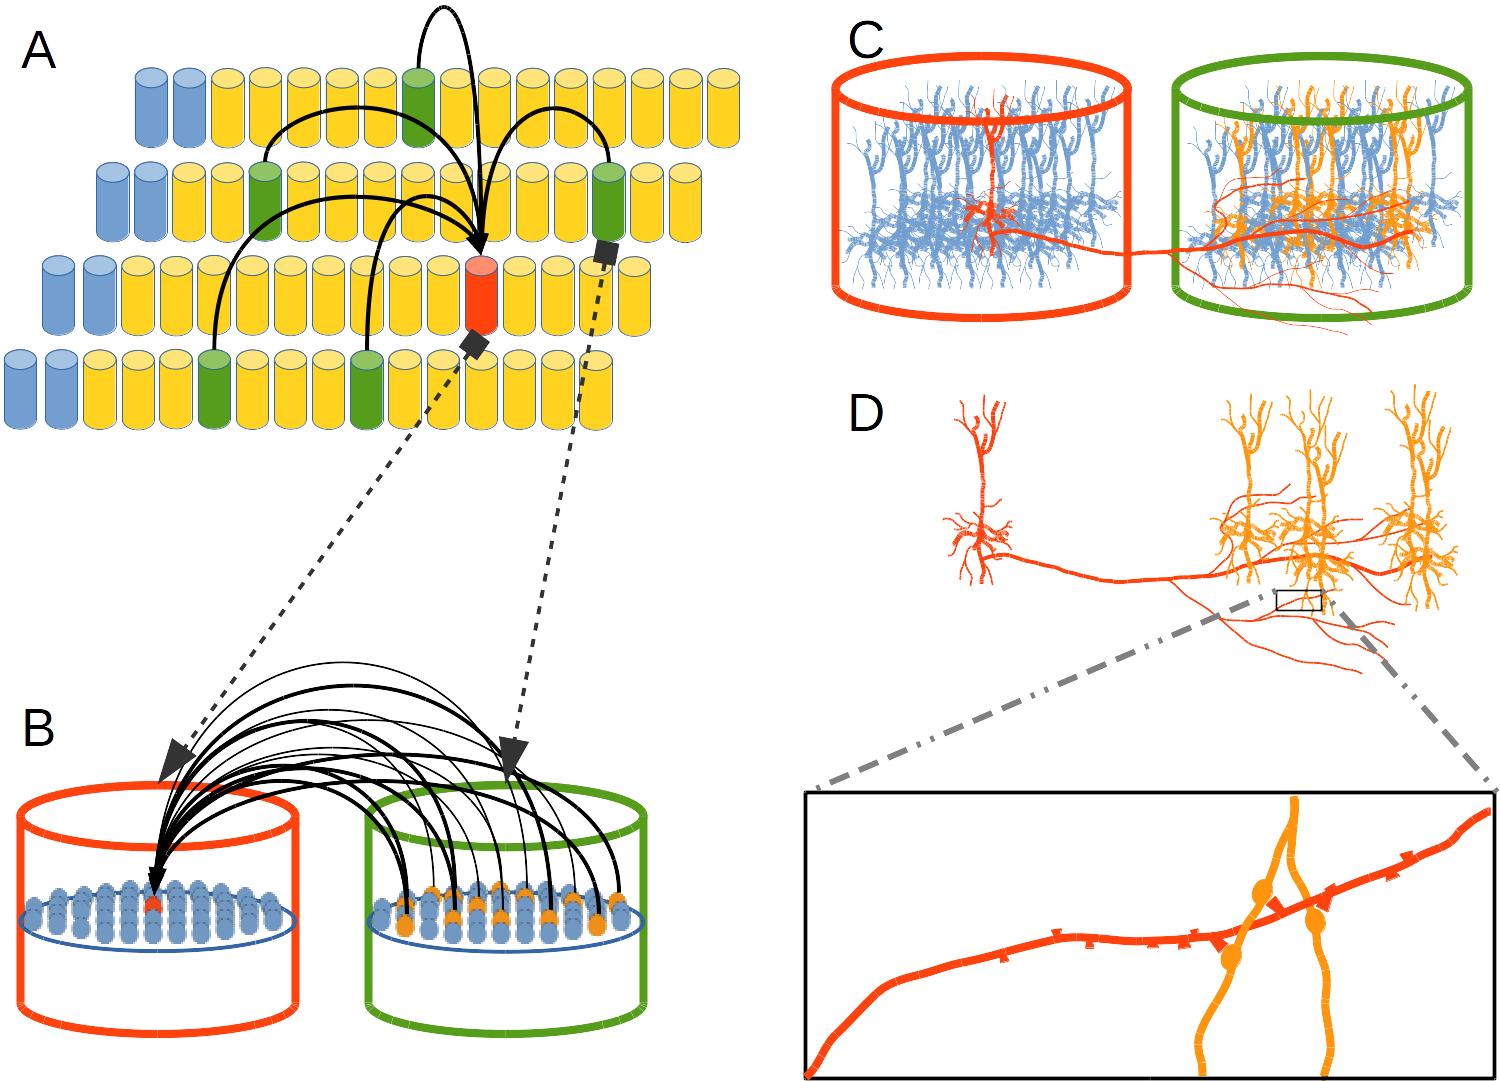
\includegraphics[width=0.8\textwidth]{DistalDendrites.png}
    \caption{Distal dendrites in the \gls{el}.
    (A) Distal dendrites can be (i) lateral, linking neighboring \glspl{cc} in the same cortical patch, and (ii) apical, which link \glspl{cc} in different cortical patches.
    (B) A distal dendritic branch between the red \gls{cc} and a green \gls{cc} entails that every neural unit in the red \gls{cc} is linked to a different subset of neural units in the green \gls{cc} by means of potential connections. The subset of potential connections comes from a percentage of neural units inside the green \gls{cc}. Such percentage is a tunable parameter for the \gls{cc}.
    (C) Physical proximity of a dendritic branch from the red cell to axonal branches from yellow cells determines potential connections which could prosper becoming in established synapses depending on the activity among cells.}
    \label{fig:DistalDendrites}
\end{figure}

A distal dendrite linking two \glspl{cc} as in Fig. \ref{fig:DistalDendrites} A implies that each neural unit in a \gls{cc}--in red in Fig. \ref{fig:DistalDendrites} B--is linked to a sub-set of units in neighboring \glspl{cc} in the same cortical patch, or in other \glspl{cc} in a foreign cortical patch, as shown in green in Fig. \ref{fig:DistalDendrites} B. Such sub-set of neural units is determined by the physical anatomical configurations of dendrites from the red neural unit in Fig. \ref{fig:DistalDendrites} B to the yellow neural units in green \glspl{cc}, as shown in Fig. \ref{fig:DistalDendrites} C.

Fig. \ref{fig:DistalDendrites} C shows how lateral dendrites extend through cortex to link a neural unit to other neural units in neighboring \glspl{cc} in the same cortical patch--the \gls{el} in our case. Apical dendrites on the other hand, receive information from \glspl{cc} located in foreign cortical patches by means of extended axons which leave their cortical domain, travelling through white matter and finally entering the \gls{el} cortical patch up to the most superficial layer of cortex called L1, where apical dendrites from local cells extend.


Fig. \ref{fig:DistalDendritesGrowth} depicts the process of synaptic growth in distal dendrites. The red square represents a \gls{cc} whose distal dendritic branches link its neural units to neural units in other \glspl{cc} in green in the figure.

\begin{figure}[h!]
    \centering
    %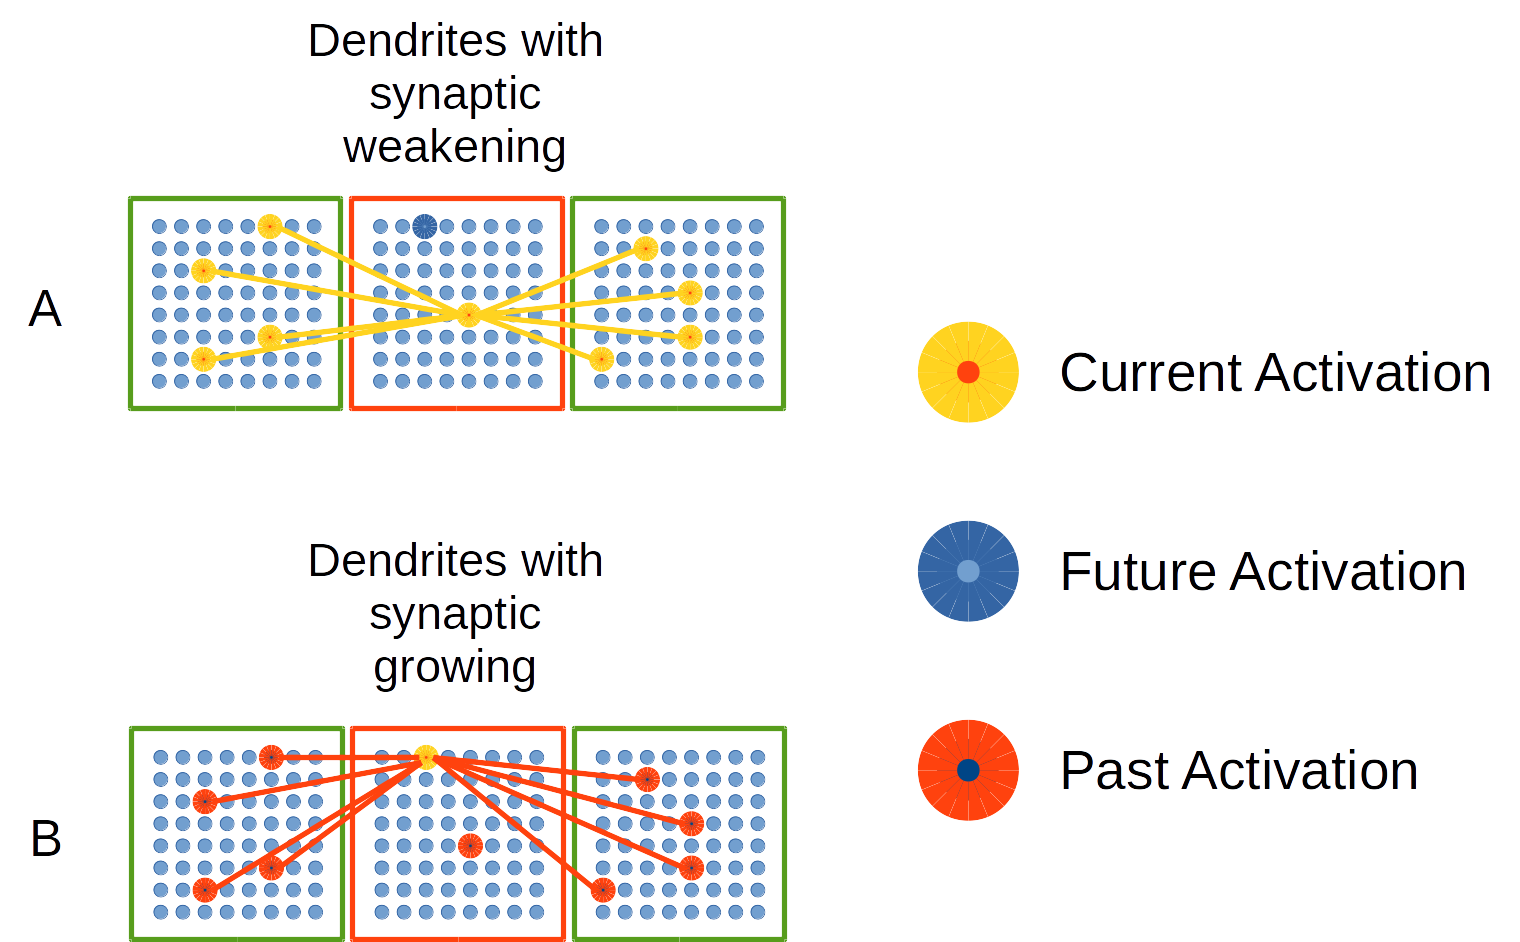
\includegraphics[width=0.8\textwidth]{DistalDendritesGrowth.png}
    \caption{Synaptic growth in distal dendrites in the \gls{el}.}
    \label{fig:DistalDendritesGrowth}
\end{figure}

 In Fig. \ref{fig:DistalDendritesGrowth} A, the current and simultaneous activation of neural units in linked \glspl{cc} decreases the synaptic strength in the potential synapses in such dendrites. In Fig. \ref{fig:DistalDendritesGrowth} B, potential synapses among currently activated neural units and past activated ones are strengthened. This mechanism of synaptic growth simulates \gls{stdp} biological processes in cortex.
 
 As already mentioned, lateral dendrites bring information from previous activity in neighboring \glspl{cc} in the \gls{el}. This adds restrictions to the activation of neural units regarding previous activation in the same area. This would produce syntactic constraints which would bias the activation of certain patterns compared to others which are less coherent regarding the statistical sequential regularities immerse in the grammatical structure of the stimuli.

Apical dendrites bring information from foreign cortical patches. In the present work, we simulate apical dendrites bringing information from \glspl{ba} 44 and 6, which are related to phonological information processing in the \gls{lifg} complex \cite{Lee3942, PMID:27381836, HEIM2003285,
PMID:18296070, AMUNTS200442}. In order to provide such information, we generate three \glspl{sdr} which supply a coarse clue to the \gls{el} about three major word categories: (i) content words, (ii) function words and (iii) verbs. We consider that phonological constraints could provide a much richer and fine-grained correlated repertoire, yet we decided to keep such constraints at a minimum in order to test the model's reaction using the minimal hint phonology could provide.
}













\iftoggle{DEBUG}{
\subsection{Activación Cortical en la \gls{el}}

}{
\subsection{Cortical Activation in the \gls{el}}

The dynamics of cellular activation in the \gls{el} is depicted in Fig. \ref{fig:Activation}. Repeated correlation among semantic afferent, sequential lateral and phonological apical constraints determines the strength of distal dendritic synapses in such a way that certain events will be more predictable than others. As long as the sequence of sentence constituents keeps a certain level of predictability with respect to the training material, activation patterns in the \gls{el} will return enough sparsity, and a phenomenon of repeated \glspl{sdr} will be sustained throughout time. When unlikely events--with respect to training material--arise, sparsity cannot be sustained by the network and a phenomenon called \gls{mfe} will emerge as a consequence of the inability of the network to correctly predict such events. As a result of the ignorance of the network to correctly predict an event, it activates all likely hypotheses given the semantic constraints. In this way, the \gls{el} loses the bias established by syntactic constraints, opening more hypotheses in order to receive subsequent lexical events in a better condition.

\begin{figure}[h!]
    \centering
    %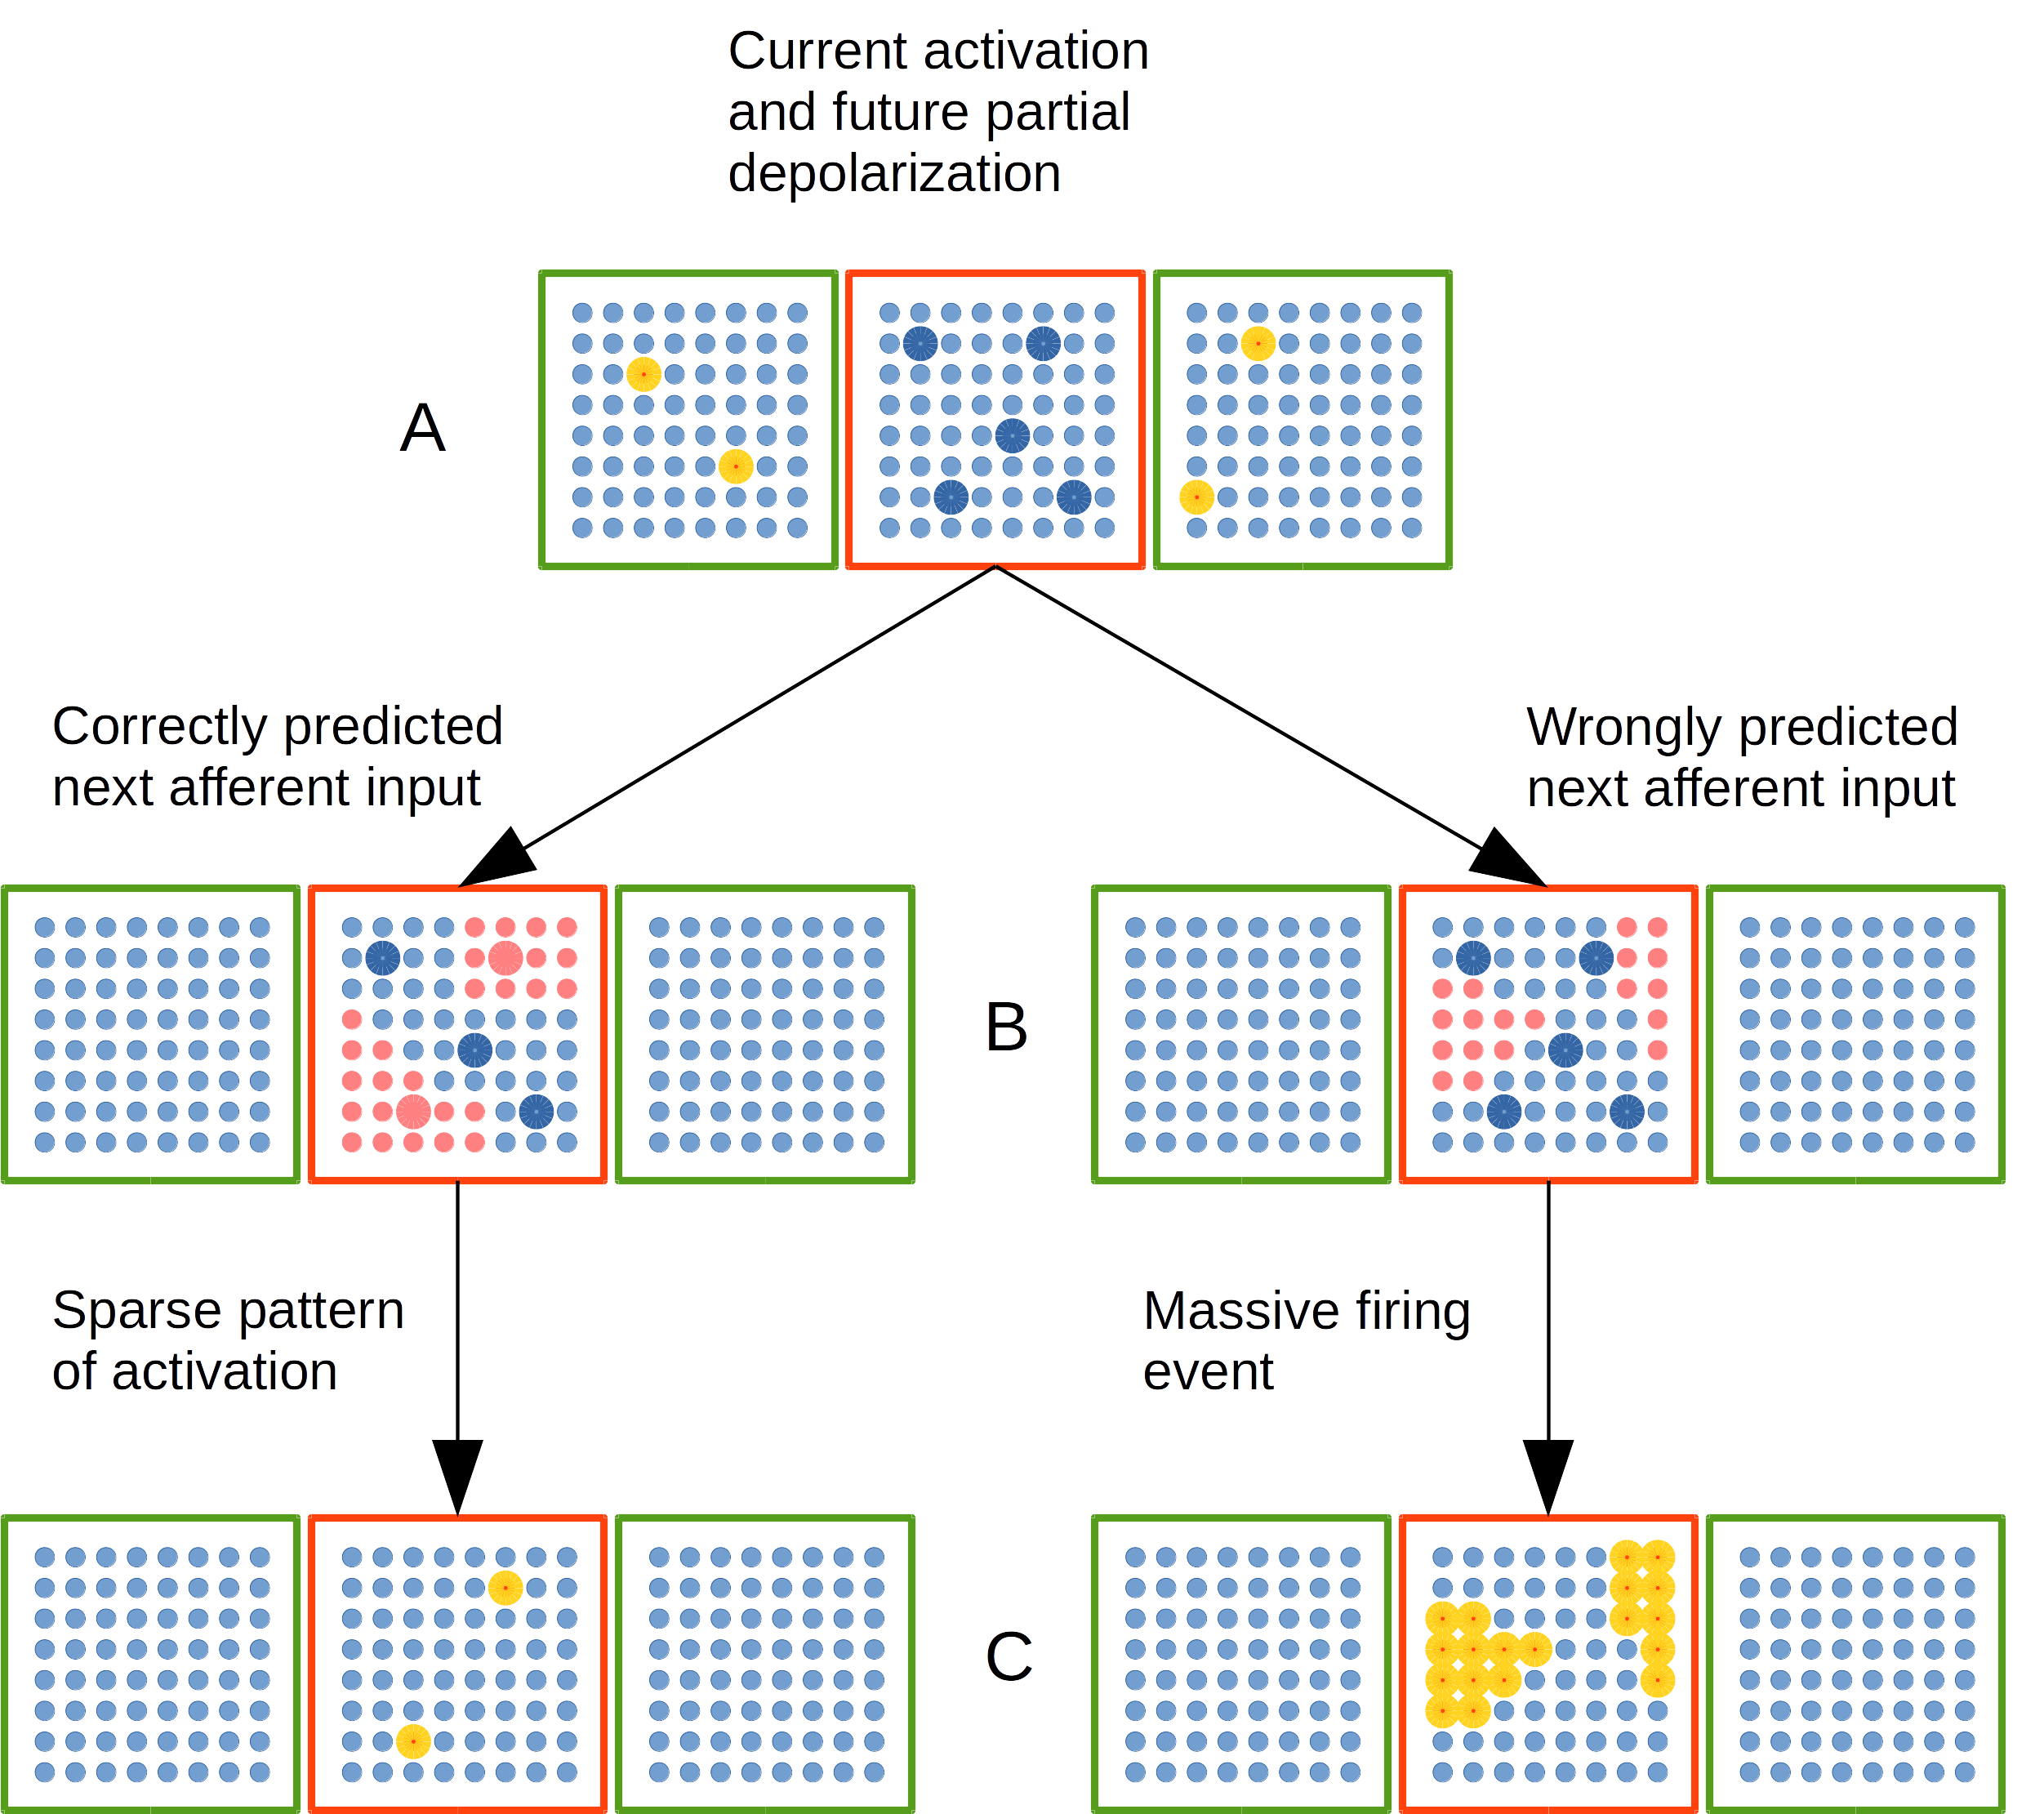
\includegraphics[width=0.9\textwidth]{Activation.png}
    \caption{Dynamic cellular activation in a \gls{cc} in the \gls{el}.
    A red cortical column is linked with two green cortical columns by means of distal dendrites.
    (A) Cellular activation in green \glspl{cc}--highlighted yellow cells--puts neural units
    in red \gls{cc} in a partially depolarized--predictive state highlighted in blue.
    (B) Cluster of neural cells activated by afferent inputs.
    Left: A substantial amount of partially depolarized cells are in the afferently excited cellular clusters.
    Right: There is no substantial amount of partially depolarized cells inside afferently excited cellular clusters.
    (C) \gls{cc} with active cellular units highlighted in yellow.
    Left: Sparse pattern of cellular activation.
    Right: Massive pattern of activation.}
    \label{fig:Activation}
\end{figure}

In Fig. \ref{fig:Activation} A, current activation of neural units in green \glspl{cc} plus distal dendritic synapses established after learning, partially depolarize specific neural units in the red \gls{cc}. Such partially depolarized units are set as predictable firing units for the arrival of the next lexical event. In Fig. \ref{fig:Activation} B, afferent semantic constraints from the next sentence constituent excite specific clusters of neural units in the red \gls{cc}. On the left, such clusters of afferently excited units contain enough partially depolarized units which will activate before rival units in the excited clusters and--as a consequence of that--will be able to inhibit rival units activation as shown in Fig. \ref{fig:Activation} C on the left. In such way, the current lexical event is correctly predicted by the network. On the right side of Fig. \ref{fig:Activation} B, the afferently exited clusters do not contain enough partially depolarized units, which implies that the great majority of the units in the clusters are in very similar conditions to fire. This circumstance determines that all the units in the afferently excited clusters will fire producing a \gls{mfe} as shown in Fig. \ref{fig:Activation} C on the right. Such event indicates that the network is not correctly predicting the sequence of lexical constituents in the sentence.
}
























\iftoggle{DEBUG}{
\subsection{Perfil Experimental}

}{
\subsection{Experimental Setup}

The experimental setup used in this paper is depicted in Fig. \ref{fig:Experiment}. Our main hypothesis is that cortical activation from the \gls{el} in response to sentence lexical constituents, will provide better information to the supervised algorithm to classify the grammatical function in such constituents than the information provided by word2vec. Therefore, we used the features delivered by word2vec and by the \gls{el} in response to each sentence constituent in order to train both classifiers shown in Fig. \ref{fig:Experiment}. Then, we tested the trained algorithms using different corpora to the one used for training.


\begin{figure}[h!]
    \centering
    %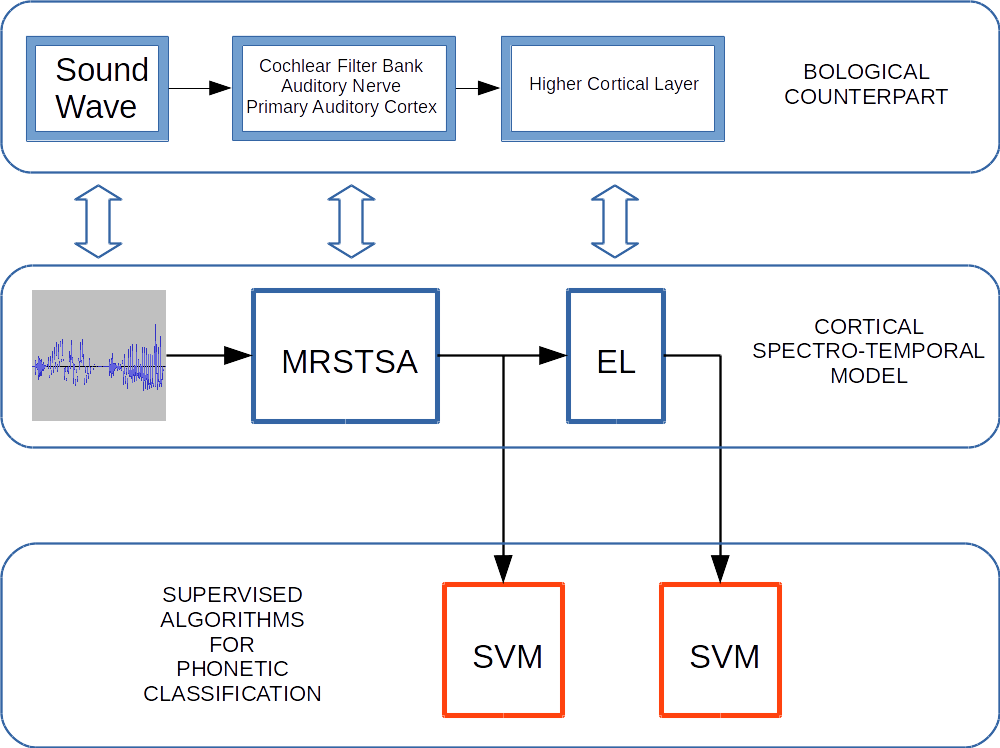
\includegraphics[width=0.8\textwidth]{Experiment.png}
    \caption{Experimental setup to test grammar classification task performances.
    Semantic constraints generated by means of word2vec are received by the \gls{el} afferent dendrites.
    Phonological constraints are \glspl{sdr} received by the \gls{el} apical dendrites.
    Grammatical word classification tasks are performed on both outputs--from word2vec and from the \gls{el}--by the \gls{svm} algorithm.
    Each section in the model has its biological counterpart.}
    \label{fig:Experiment}
\end{figure}

We used supervision by means of the \gls{svm} classification method, receiving the outputs from each algorithm. We did this to test the generalization properties in the grammatical features abstracted by the \gls{el} in comparison with the grammatical features returned by word2vec (Fig. \ref{fig:Experiment}). In the present work, we used a package called \gls{libsvm} \cite{CC01a, libsvm}. We trained and tested the \gls{svm} classifiers using 5-fold cross-validation, and configured them to use a linear kernel with one parameter $C$, which we swept to find the best trained model for each classifier.

We implemented an \gls{el} with 225 \glspl{cc} arranged in a two-dimensional array of 15 by 15 \glspl{cc}. Each \gls{cc} was automatically distributed using individual locations along its afferent, lateral and apical inputs in a uniform way. Each \gls{cc} received afferent information by means of two-dimensional afferent receptive fields of 9 by 29 components centered at individual locations over a 10 by 30 word2vec space. We enabled the wraparound property in order to make each receptive field span the entire word2vec array. We also instructed each column to receive only 31 inputs, which is a minor percentage of such receptive field. Individual afferent inputs for each \gls{cc} were chosen randomly during the \gls{el} initialization process.

For this model instance we implemented distal lateral and apical dendritic branches. We configured each \gls{cc} to have a lateral receptive field with 9 by 9 neighboring \glspl{cc}
and to receive information from 72 of the 81 \glspl{cc} in the receptive field--a 90\% of the receptive field. In reference to apical dendrites, we configured each \gls{cc} to have an apical receptive field of 11 by 11 foreign \glspl{cc} and to receive information from 108 of the 121 \glspl{cc} in the receptive field--also a 90\% of the receptive field.

Each \gls{cc} was composed of a two-dimensional array with 15 by 15 (225) neural units and each unit in a column could be potentially connected with only 6 neural units from each linked neighboring column. Each neural unit in a \gls{cc} ended up with 72 lateral dendritic branches with 6 potential connections each (432 distal lateral potential synapses per cellular unit) and with 108 apical dendritic branches with 6 potential connections each (648 distal apical potential synapses per cellular unit). That is, each neural unit in a \gls{cc} ended up having 1080 distal potential synapses. Such potential synapses were randomly chosen for each neural cell and for each dendritic branch in the cell during the Encoder initialization procedure. The \gls{el} consisted of 50625 cellular units with 1569375 proximal synapses and 54675000 distal synapses. It is important to highlight that distal synapses represented potential connections from which only a small percentage had a significant synaptic weight as to be considered as an established connection. Weak synapses were periodically pruned by means of homeostatic processes in the network, leaving distal dendrites with a sparse connectivity in the receptive fields. The sparseness in such connectivity matrices could exceed 90\%.

The fictitious \gls{cl} from which the \gls{el} received apical constraints--in the form of phonological \glspl{sdr}--had the same columnar and cellular configuration than the \gls{el}.

The training procedure consisted of 2 stages and for each stage the \gls{el} received the same corpus twice. During each learning stage, certain parameters--such as the learning rates in proximal and distal synapses and the lateral intra-column interaction--were exponentially and progressively decreased from an initial value. The same parameters were also decreased for each successive stage. An additional stage was executed with the learning parameters fixed.

The sparsity in the activation for each \gls{cc}--even \glspl{cc} in the phonological \gls{cl}--was 99\% (just 2 neural units out of 225 could be active for normal activation events). On the other hand, the afferent excitation affected 10\% of the units inside the clusters in each \gls{cc} (22 neural units, which could be activated in case of a \gls{mfe}; Fig. \ref{fig:Activation}).

In order to train the model we used a corpus from the WikiSplit dataset by Google \cite{BothaEtAl2018}. This dataset was constructed automatically from the publicly available Wikipedia revision history. The complete dataset contains one million English sentences, each split into two sentences that together preserve the original meaning, extracted from Wikipedia edits. In order to train the model we used a corpus called \texttt{test} from the dataset. The corpus has 14980 sentences. We cleaned the corpus erasing punctuation marks to get a file in which each sentence is a sequence of individual words in a line.

We tagged each word in the corpus with its grammatical function in the sentence context. To that end we used Enju natural language parser for English (Enju 2.4.4 Copyright (c) 2005-2010, Tsujii Laboratory, The University of Tokyo). This parser has a wide-coverage probabilistic \gls{hpsg} \cite{Yusuke:2002:MEE:1289189.1289214, noauthor_2_nodate, Miyao2004CorpusOrientedGD, Miyao:2005:PDM:1219840.1219851, Ninomiya:2006:ELM:1610075.1610100, Ninomiya:2007:LMN:1621410.1621418, Miyao:2008:FFM:1350986.1350988}, as well as an efficient parsing algorithm \cite{tsuruoka:2004b, Ninomiya:2005:EBT:1654494.1654505, bc22fe91f8a743269f26f92abfd79790, Matsuzaki:2007:EHP:1625275.1625546}.

Enju can effectively analyze syntactic/semantic structures of English sentences and provide the user with phrase structures and predicate-argument structures. Those outputs would be especially useful for high-level \gls{nlp} applications, including information extraction, automatic summarization, question answering, and machine translation, where the "meaning" of a sentence plays a central role \cite{noauthor_english_2019}. 

We analyzed the complete corpus grammatically by means of Enju in its stand-off format. In this format, the span of each tag is represented with the position in the original input sentence, each line representing a tag.  The label of a tag (e.g. "\texttt{cons}" and "\texttt{tok}") is output first, and the rest represents the attributes. A constituent is tagged by \texttt{cons} while each word is tagged by \texttt{tok}. The attribute "\texttt{cat}" represents the phrase symbol of the constituent. The attribute "\texttt{pos}" represents a part-of-speech and--inside \texttt{tok}--the attribute \texttt{cat} represents the same information as in \texttt{cons}.

To tag the grammatical function of the words in each sentence we used part of the information returned by Enju. We specifically used \texttt{tok} tags from which we extracted the attributes \texttt{cat} and \texttt{pos}. The conjunction of those two attributes formed the grammatical function with which we tagged each word in the sentence context for all the corpus. In this way, we ended up having 113 different grammatical categories. 

Once we had all the words in the corpus tagged, we synchronized apical \glspl{sdr} in the training stage in such a way that nouns, adjectives and adverbs were correlated with the \emph{content word} \gls{sdr}. Articles, auxiliaries, demonstratives, quantifiers, prepositions, pronouns, conjunctions, etc, were correlated with the \emph{function word} \gls{sdr}, and the rest of the tagged words were correlated with the \emph{verb} \gls{sdr}.

First, we trained the model, and then we ran it in inference mode. In such mode, the \gls{el} processed the information with its learning properties disabled. In this manner, during inference, the \gls{el} did not modify its synapses and just returned patterns of activation in response to the stimuli it received. We then used the outputs from word2vec and from the \glspl{el} in inference mode to train the \gls{svm} classifiers using the grammatical tags we obtained from Enju.
}






















\iftoggle{DEBUG}{
\section{Resultados}

}{
\section{Results}

We used the outputs from word2vec and from the \gls{el} in inference mode to train the \gls{svm} classifiers shown in Fig. \ref{fig:Experiment}. We used the outputs from such algorithms in response to 150, 300 and 600 sentences from the corpus. The cross validation training performances are shown in Table~\ref{SVM_Training}.

\begin{table}[h!]
\centering
\caption{\gls{svm} 5-fold cross validation training results}
\begin{tabular}{|l|l|l|}
\hline
                & word2vec  & Encoder Layer \\ \hline
150 Sentences   & 84.03\%   & 89.40\%       \\ \hline
300 Sentences   & 83.35\%   & 90.47\%       \\ \hline
600 Sentences   & 80.96\%   & 90.79\%       \\ \hline
\end{tabular}
\label{SVM_Training}
\end{table}

We then tested the classification accuracy of each \gls{svm} algorithm--the one trained using 150 sentences, the one trained using 300 sentences and the one trained using 600 sentences--using the outputs from word2vec and the \gls{el} in response to different sentences--not used to train the classifiers. We did so for 10 different sets of sentences in each case--i.e. 10 different corpora with 150 sentences, 10 different corpora with 300 sentences and 10 different corpora with 600 sentences. %Table \ref{SVM_Testing} shows the average classification performances returned by the tests in each case.

%\begin{table}[h!]
%\centering
%\caption{\gls{svm} average testing results}
%\begin{tabular}{|l|l|l|}
%\hline
%                & word2vec  & Encoder Layer \\ \hline
%150 Sentences   & 70.18\%   & 78.59\%       \\ \hline
%300 Sentences   & 73.48\%   & 81.32\%       \\ \hline
%600 Sentences   & 74.30\%   & 83.10\%       \\ \hline
%\end{tabular}
%\label{SVM_Testing}
%\end{table}

Fig. \ref{fig:PLOT} shows the average classification accuracy returned by the tests in each case--i.e. 150, 300 and 600 sentences corpora. 

\begin{figure}[h!]
    \centering
    %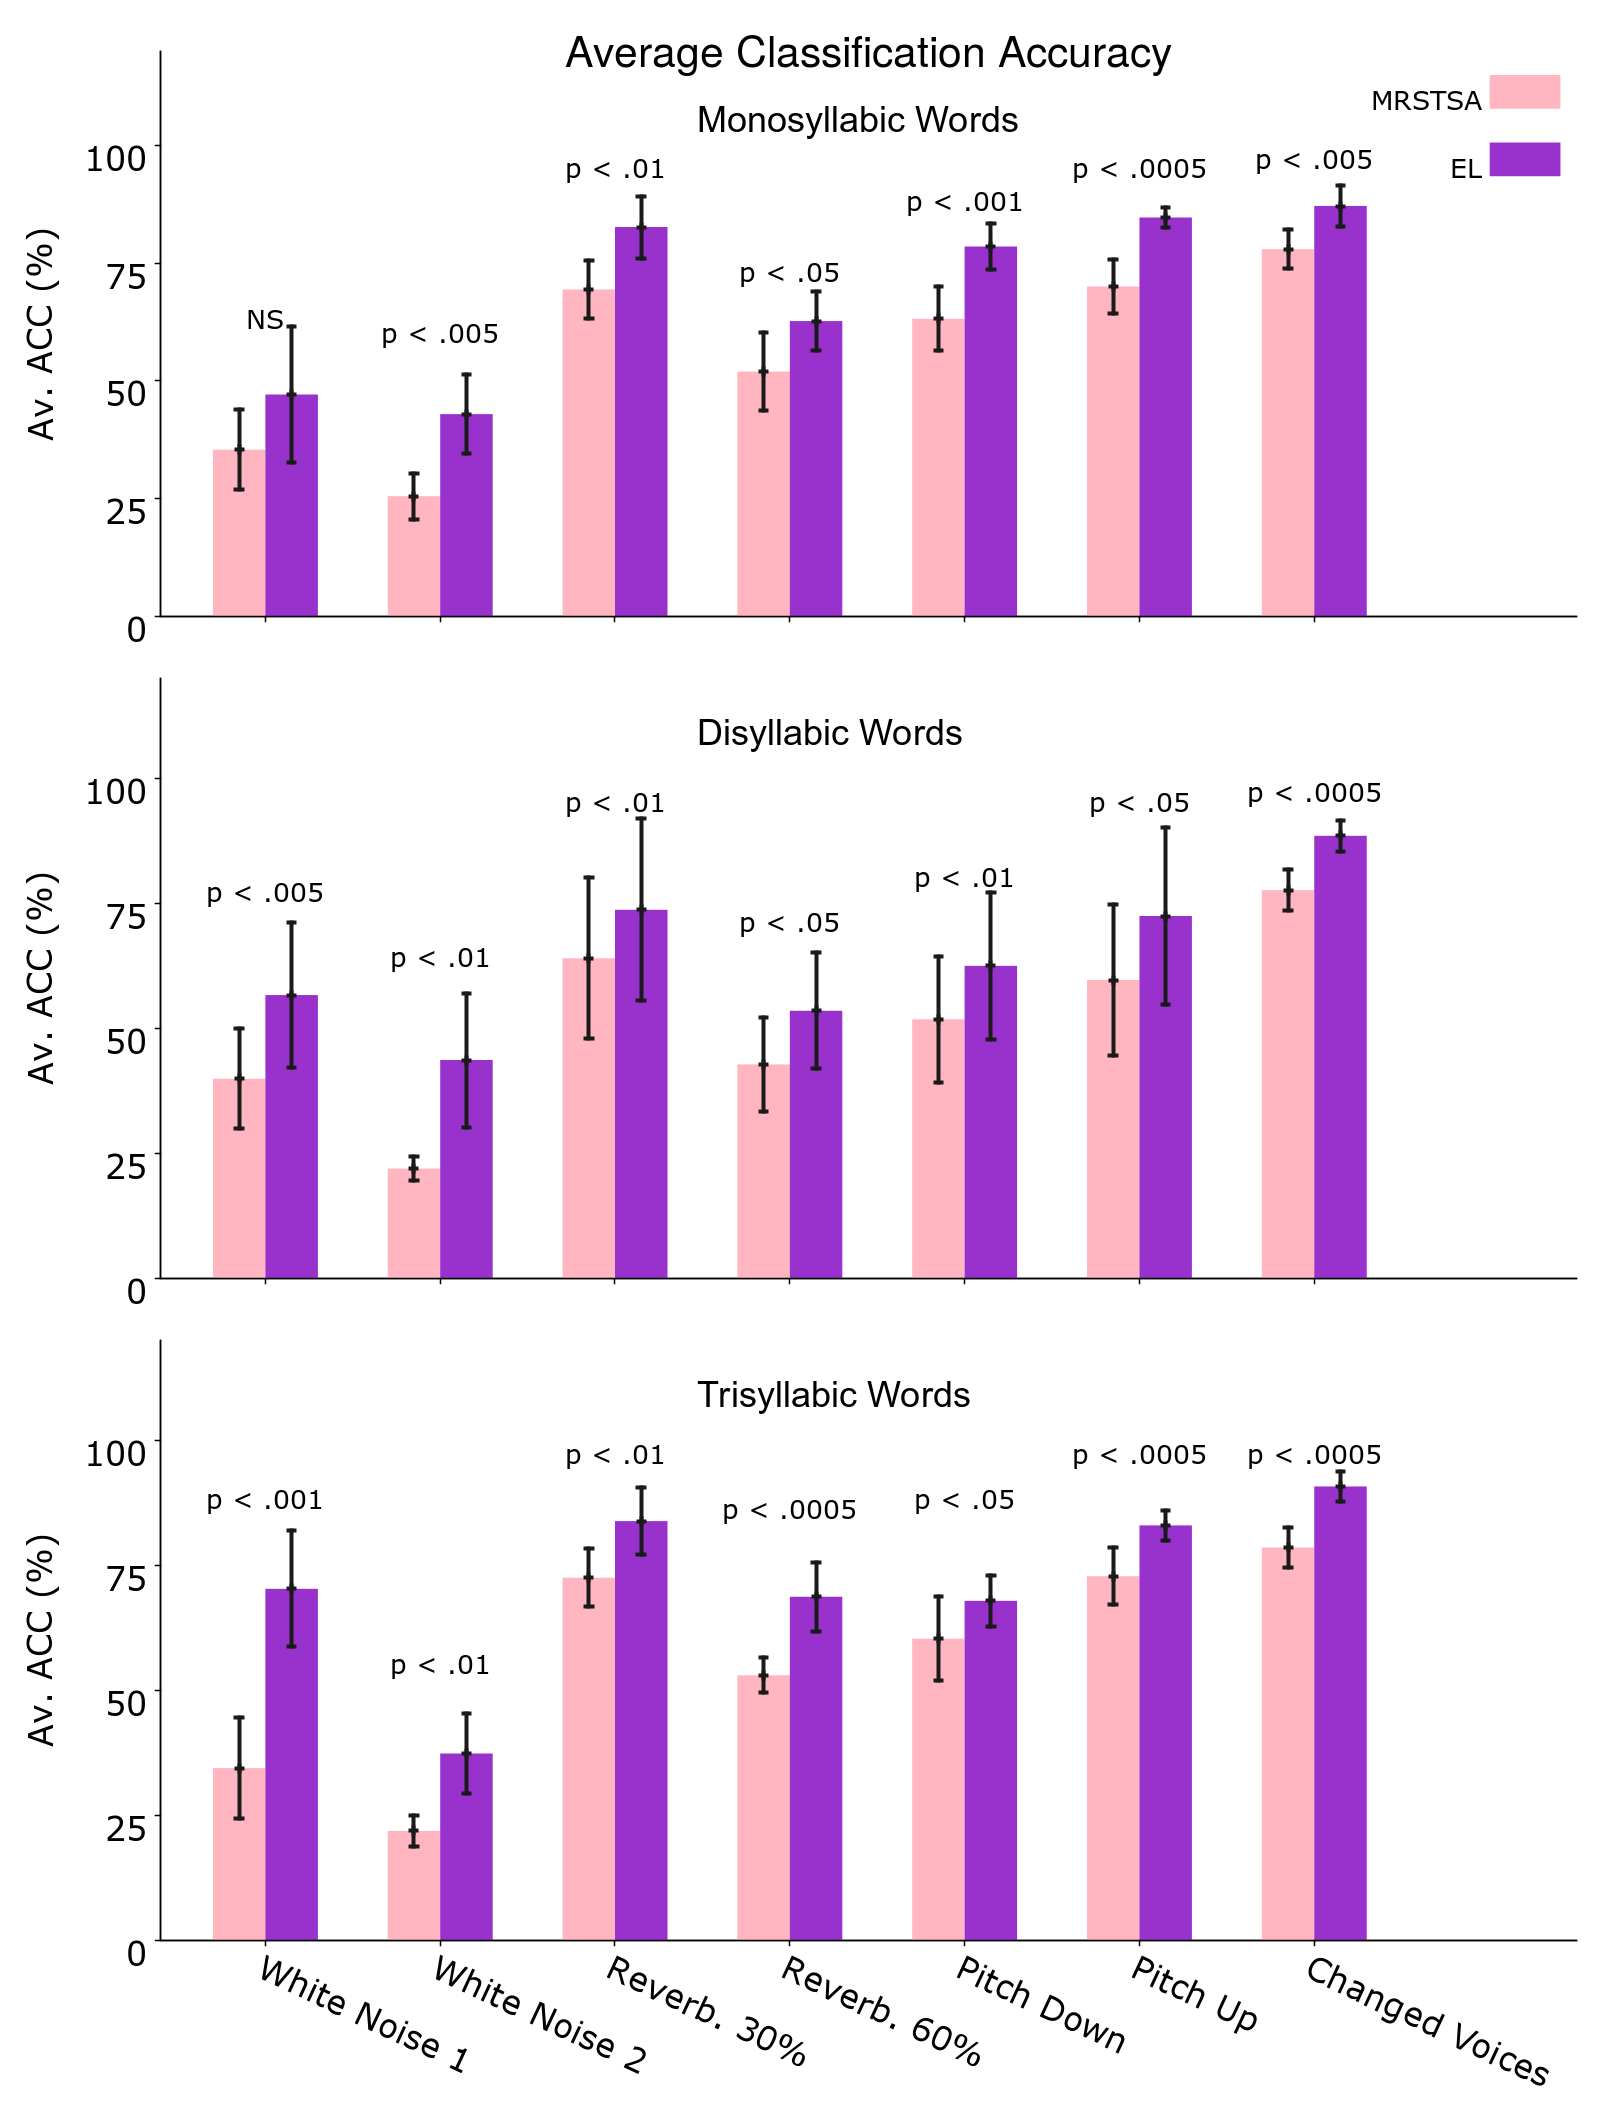
\includegraphics[width=1.0\textwidth]{PLOT.png}
    \caption{Grammatical Average Classification Accuracy. Average classification accuracy of features returned by word2vec vs. features returned by the \gls{el} for three experimental conditions. The \emph{p} values correspond to two-tailed paired t-tests (Holm-Bonferroni validated); each for 10 different corpora. Error bars depict 95\% Confidence Interval values.}
    \label{fig:PLOT}
\end{figure}
  
We performed two-tailed paired t-tests for 10 different corpora from the dataset. Given that we conducted 3 t-tests for the grammar classification task (i.e. 150, 300 and 600 sentences), we performed Holm–Bonferroni corrections with a correction factor of 3 in order to reduce the probability of
type I and type II errors in the tests \cite{10.1093/biomet/75.2.383}. As can be seen in Fig. \ref{fig:PLOT} the \gls{el} performed significantly better than word2vec in all the experimental conditions.
}


















\iftoggle{DEBUG}{
\subsection{Análisis de una Oración Individual}
\label{SentenceAnalysis}

}{
\subsection{Individual Sentence Analyses}
\label{SentenceAnalysis}

With the aim of illustrating the results showed by Fig. \ref{fig:PLOT}, Fig. \ref{fig:Sentence1} shows how word2vec and the \gls{el} serve \gls{svm} algorithms for grammar classification tasks within the context of the sentence: \texttt{wolves feed primarily on medium to large sized ungulates though they are opportunistic feeders and will generally eat any meat that is available}. In Fig. \ref{fig:Sentence1} we highlight specific words in the sentence and show how \gls{svm} models classify them using the information produced by each algorithm.

\begin{figure}[h!]
    \centering
    %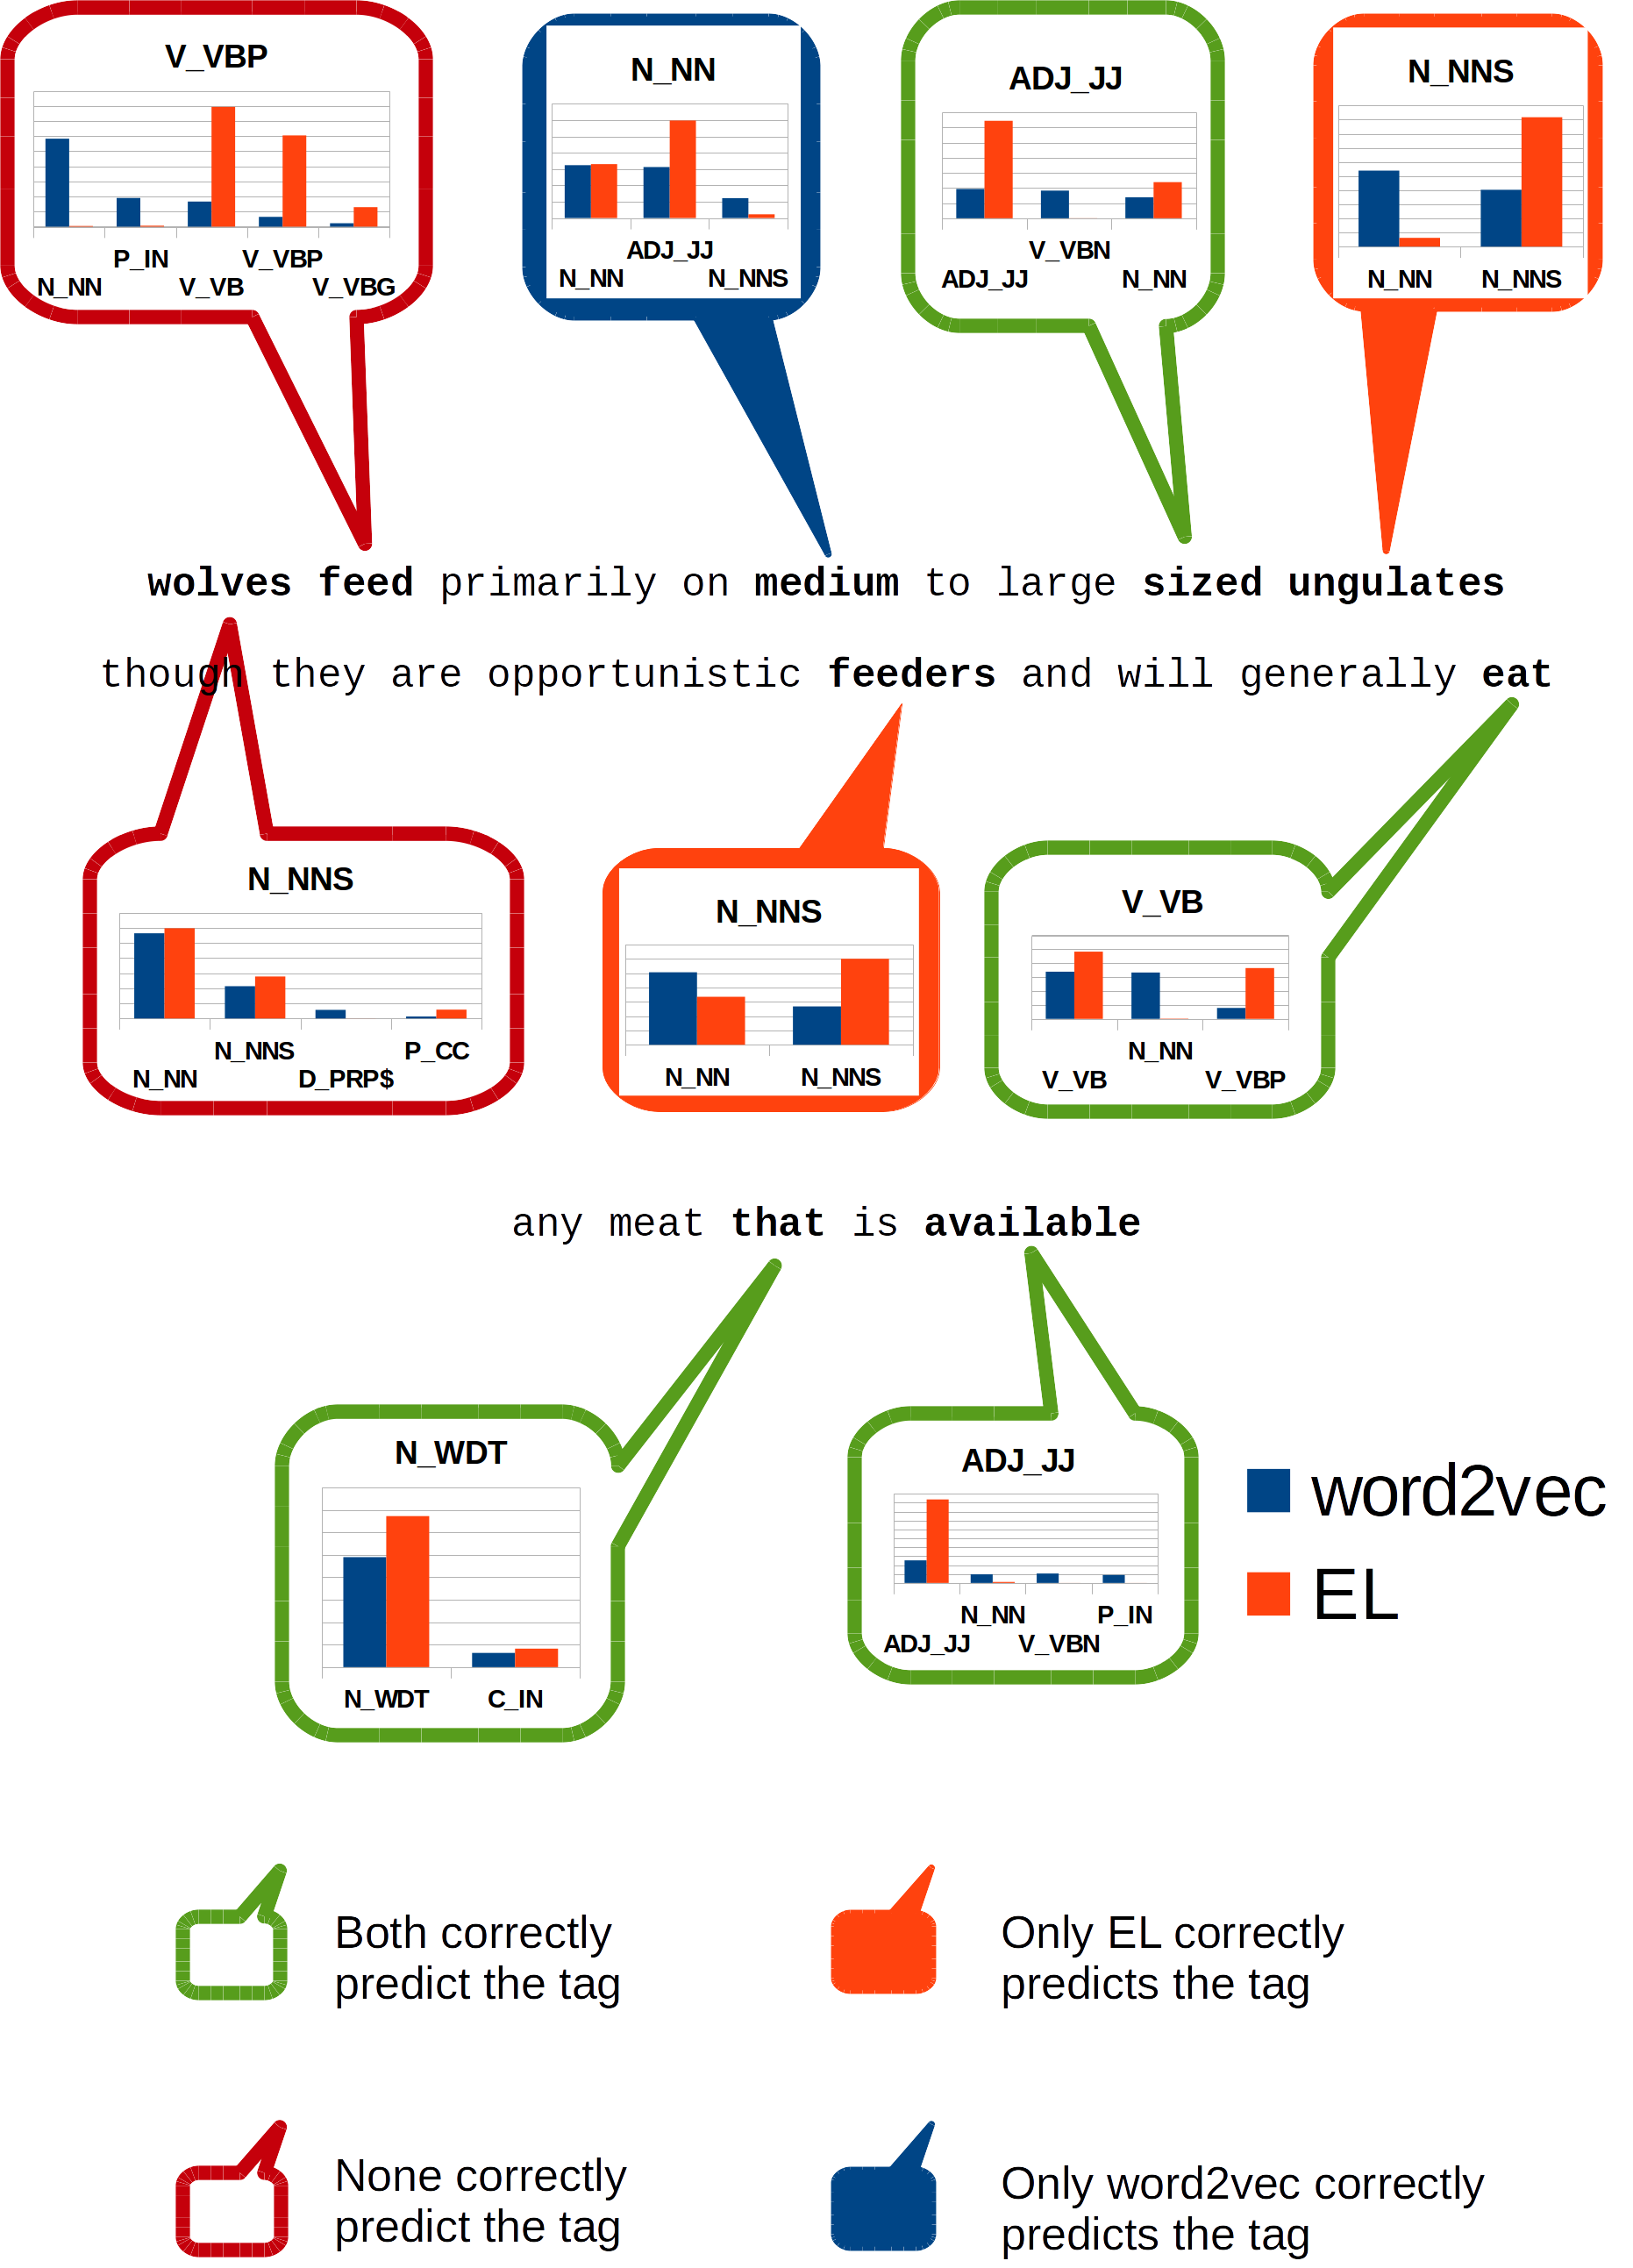
\includegraphics[width=0.9\textwidth]{Sentence1.png}
    \caption{Classification of individual constituents within the sentence: \texttt{wolves feed primarily on medium to large sized ungulates though they are opportunistic feeders and will generally eat any meat that is available}.}
    \label{fig:Sentence1}
\end{figure}

The first word (\texttt{wolves}) is incorrectly classified by both algorithms losing the number sense in the lexical entry which is correctly detected by our gold standard --Enju. The second word (\texttt{feed}) is a verb, non-3rd person singular present according to our gold standard. Both algorithms incorrectly classified such constituent too, but this time there was a clear difference regarding the information each algorithm provided the classifiers. On the one hand, word2vec provided features to which the classifier assigned a maximum of 29\% likelihood of being a singular noun. On the other hand, the \gls{el} provided features to which the classifier assigned 39\% chance of being a verb in base form, but it also assigned 30\% likelihood to the same tag assigned by the gold standard--which is the correct one for this case.

The word \texttt{medium} which clearly acts as an adjective in this sentence, is missclassified by our gold standard as a singular noun; hypothesis to which word2vec endorses. Nonetheless, the \gls{el} provides information to the \gls{svm} such that it assigns almost 60\% probability that this sentence constituent is an adjective.

The word \texttt{sized} acts as an adjective in this sentence too. This constituent is correctly classified by both algorithms, but the \gls{el} provides activation which gives the \gls{svm} algorithm more than 64\% confidence about its classification, while word2vec provides features that turns the \gls{svm} classification considerably more undetermined: it assigned 19\% to the correct tag, but in addition it also assigned 18 and 13\% to the tags "verb in past participle" and "singular noun" respectively.

In the words \texttt{ungulates} and \texttt{feeders} the \gls{el} provided enough information to the \gls{svm} algorithm as to make it assign a high probability--more than 90\% for ungulates and more than 60\% to feeders--to the correct tags in both cases. On the other hand, word2vec lost the number sense attributing a singular noun tag to both constituents.

The word \texttt{eat} is correctly classified by both algorithms but the \gls{el} assigns the highest probability to the correct tag--more than 48\%--while word2vec spreads chance out along a larger range of tags including nouns.

Finally, the word \texttt{available} was correctly classified by both algorithms, but the \gls{el} assigned by far the highest probability to the correct tag--more than 93\%--while virtually neglecting alternative tags as viable options. On the other hand, word2vec assigned a scarce 25\% chance to such tag, distributing the probability throughout a much larger range of tags.
}

























\iftoggle{DEBUG}{
\section{Discución}

}{
\section{Discussion}

In this paper we introduce a computational model inspired in specific features found in brain cortex whose outcome mimics the selection mechanisms proposed in the \glsfirst{uf}\cite{Hagoort2005OnBB}.

By means of the experimental results presented here we show how the convergence of linguistic constraints from different sources, improves the classification of grammatical functions carried by constituents within a sentence context.

For instance, when analyzing a specific sentence, both algorithms lose number sense in the first word (\texttt{wolves}). Except for such case, the \gls{el} catches the number sense in the rest of the cases in which plural nouns appear (\texttt{ungulates} and \texttt{feeders}), while word2vec continues losing number sense in those examples too. In our implementation, phonological constraints from apical dendrites do not provide enough information to the \gls{el} to make such distinction. Syntactic constraints coming from lateral dendritic activation within the sequence of constituents, fulfil the information needed by the \gls{el} to constraint the choices among different unification options. In such way, the \gls{el} ends up activating only the most suitable option given the information received. In this example, semantic information from word2vec does not suffice to distinguish the number attribute in nouns, but the incorporation of syntactic constraints such as the adjectives preceding nouns seems to bias the probability towards the plural attribute. Furthermore, larger distance dependencies such as the word \texttt{are} in the phrase \texttt{are opportunistic feeders}, could have influenced the classification given the sequential properties incorporated in the \gls{el} \cite{Cui:2016:COS:3030654.3030660}. Since syntactic constraints do not appear in the first word of the sentence, the \gls{el} makes the same kind of mistake than word2vec, and neither semantic nor phonological constraints provide sufficient information as to catch the plural attribute in the noun.

The classification of verbs in the sentence (\texttt{feed} and \texttt{eat}), clearly shows the importance of phonological constraints from apical dendrites. In such regard, word2vec confers a very high weight to nouns in both examples, completely misclassifying the word \texttt{feed} as a singular noun and giving almost the same probability (33.9\% vs. 33.3\%) to the tags verb in base form and singular noun when the verb \texttt{eat} appears. The \gls{el} on the other hand, virtually disregards the classification of such verbs as nouns, misclassifying \texttt{feed} as a verb in base form although providing a high chance to the correct tag (the second highest). The \gls{el} also produces a correct classification of \texttt{eat}, providing a high probability to the correct tag.

Adjectives are quite remarkable as can be seen in Fig. \ref{fig:Sentence1}. Even though the adjectives \texttt{sized} and \texttt{available} are correctly classified by both algorithms, there is a notorious difference in such classifications which can be appreciated in the soundness with which the \gls{el} attributes chances to the correct tag in both cases. On the other hand, word2vec is  indeterminate, attributing a very low chance to the correct tag, especially in the case of \texttt{sized}, in which the algorithm attributes almost the same probability to the tags adjective, verb in past participle and singular noun. Another important example is given with the word \texttt{medium}. Even when the appearance of such word counts as a success for word2vec, the reality is that the \gls{el} produces a correct classification of it as an adjective, and such classification is sound due to the high probability assigned to the tag.

Compared to word2vec, the \gls{el} activates fewer phrasal configurations, narrowing down the spectrum of alternative binding candidates. It assigns higher probability values to fewer tags and generally such tags are the correct ones or closer to the correct ones. This fact is supported by the higher hit rate of the \gls{el} compared to word2vec (Fig. \ref{fig:PLOT}).

A computational model that assigns thematic roles to sentence constituents has been previously developed by John and McClelland \cite{STJOHN1990217}. The model disambiguates words, instantiates vague words, and elaborates implied roles. Recently, this computational approach was used to explain the N400 event-related brain potential presenting a computationally explicit account for the emerging representation of sentence meaning \cite{rabovsky_modelling_2018}. The model succeeded capturing diverse empirical neural responses, showing that essential aspects of human language processing can be effectively represented by a proper connectionist approach. Nevertheless, the model lacked a detailed mapping of neurophysiological characteristics in cortical dynamics and used optimization algorithms (i.e. backpropagation) which are difficult to map in neural tissue.

Dominey et al. cite{Dominey2009NeuralNP} on the other hand, incorporated the functional neurophysiology of sentence comprehension (along with non-linguistic sequence processing), in a neural network model whose architecture was constrained by \gls{cstc} neuroanatomical connectivity and functional imaging data. The model was able to learn and perform several types of language and artificial syntax tasks. Their approach includes the interaction among several \glspl{ba} involved in language processing--such as \gls{ba} 47, 45 and 44/6 in the \gls{lifg}. Nonetheless, such model is also forced to choose the correct options through supervised error-driven learning methods. Such methodology, assumes the existence of internal \emph{teaching signals} in the brain. Teaching signals are needed to force the output layer to the correct answer, enabling the network to backpropagate the errors.

Michalon et al. \cite{michalon_meaning-driven_2019} developed an explicit algorithmic implementation of a parallel processing architecture that explains how syntactic and semantic information processing can interact selectively during language comprehension. The architecture advances towards the organization of language in the brain focusing in the articulation between syntax and semantics and the essence of prediction in language comprehension. The work is clearly inspired by the psychology and neuroscience of language, but it does not incorporate biologically accurate features of neural computation in its implementation.

In the present work the computational model developed, is inspired in the biology of the mammalian neocortex and simulates cortical tissue incorporating columnar organization, spontaneous micro-columnar formation, \glspl{sdr} derived from partial \gls{nmda} depolarization and adaptation to contextual activation. In addition, different roles to proximal and distal dendritic configurations simulating pyramidal cells are assigned. We incorporate important physiological and anatomical phenomena, such as the consideration of dendritic branches as active and independent processing elements, the stochastic activation of brain cells and \glspl{mfe} originated by prediction failures in the network manifesting as the activation of many neurons in a \gls{cc} impairing \glspl{sdr} formation--among others. Most \glspl{ann}, such as those used in previous works \cite{STJOHN1990217, rabovsky_modelling_2018, Dominey2009NeuralNP, michalon_meaning-driven_2019}, use artificial neurons without considering active dendrites and with an unrealistic low number of synapses, thus missing fundamental functional properties present in the brain. Furthermore, unlike established computational models, the model presented here does not incorporate optimization methods such as those found in supervised or reinforced algorithms. Even though influential research lines underpin the idea of \emph{credit assignment} supporting backpropagation processes in cortex \cite{10.7554/eLife.22901}, so far there is not enough evidence to justify the inclusion of such complex process in the brain. Moreover, our concerns regarding backpropagation in brain tissue go beyond the complexity of its algorithmic implementation. These implementations require the existence of teaching signals. Although there is evidence that animals can represent desired behavioral outputs with internal goal representations \cite{gadagkar_dopamine_2016}, it is unknown whether teaching signals indeed exist in the brain.

In the present work, we replace \emph{teaching signals} used in other systems--specially needed by backpropagation-like optimization--by the uniform and simple correlation of \glspl{sdr} activation coming from different cortical patches. Our hypothesis is that when noise is impairing the smooth individualization of a pattern coming from one source, the brain correlates such information with information coming from other sources in which the noise has not been too detrimental for the pattern that the subject seeks to classify. In the present model, when semantic information from afferent dendrites is not sufficient for grammatical disambiguation of a sentence constituent, phonological information from apical dendrites helps in such disambiguation. In the case that phonological clues cannot compensate the lack of semantic information, syntactical constraints from lateral dendrites finally come in handy. Functional connectivity across different cortical areas has been shown to facilitate speech comprehension when the intelligibility of the speech signal is reduced~\cite{Obleser2283}.

Many other sources of information--which turn out to be useful for early infant language acquisition--have not been yet considered in our computational approach. For instance, it has been shown that iconic gestures boost speech comprehension under adverse listening conditions \cite{HOLLE2010875}. Neurocognitive studies of motor representations of speech sounds, action-related language, sign language and co-speech gestures are also tightly coupled to the language system \cite{Willems2007NeuralEF}. Future work in the model will be directed towards integrating information from more sources than the ones presently used. We will also enrich phonological information from apical dendrites and procure a more holistic linguistic integration. To that end we will incorporate linguistic structures such as those supplied by FrameNet \cite{noauthor_about_nodate}. Finally, for future developments of this work, we will add reinforced mechanisms to the model, including neuromodulator-like effects in the algorithm which could significantly enhance performance.
}
























\iftoggle{DEBUG}{
\subsection{Conclusión}

}{
\subsection{Conclusion}

This research brings a novel explanation of how grammar could emerge from the interaction of specific areas in the human brain. These areas present a linguistic processing gradient which is precisely mapped in the cortical dynamics of a computational approach which simulates particular characteristics evaluated as suitable for linguistic computations in human neocortex.
We introduce a biologically plausible computational model which incorporates specific features from the mammalian cortex. Our model utilizes Hebbian-like rules without involving optimization mechanisms extensively used in prevalent \glsfirst{ml} algorithms, but of difficult justification in cortical tissue. We use such model to explain unification operations at semantic, syntactic and phonological levels of language on the cortical \glsfirst{lifg}. We show how cortical \glsfirst{sdr} activation features returned by our model are better suited to attain classification of lexical grammatical functions of words than the features returned by word2vec.
%The relevance of this research is based on its biological plausibility positioned on specific dynamical cortical features found in mammals. The simplicity of our approach stands on the fact that it does not introduce optimization mechanisms extensively used in prevalent \glsfirst{ml} algorithms, but of difficult justification in cortical tissue.
%In future versions of this work we will promote the integration of more linguistic clues, from different modalities as well as a more elaborated and refined embodiment of the current linguistic features presented here. We will also implement reinforcement learning mechanisms inspired in subcortically generated neuromodulators in the brain.
We evaluate this research as valuable for future and more brain-inspired \gls{ml} applications of \gls{nlp} as well as a complementary validation for psycho-linguistic theories of language processing. 
}






